% Created 2016-05-26 to. 16:38
\documentclass[presentation]{beamer}
\usepackage[utf8]{inputenc}
\usepackage[T1]{fontenc}
\usepackage{fixltx2e}
\usepackage{graphicx}
\usepackage{longtable}
\usepackage{float}
\usepackage{wrapfig}
\usepackage{rotating}
\usepackage[normalem]{ulem}
\usepackage{amsmath}
\usepackage{textcomp}
\usepackage{marvosym}
\usepackage{wasysym}
\usepackage{amssymb}
\usepackage{capt-of}
\usepackage{hyperref}
\tolerance=1000
\usepackage{minted}
\usepackage{tikz}
\usepackage{parskip}
\usepackage{color}
\usepackage{listings}
\usepackage{minted}
\usemintedstyle{emacs}
\usepackage{minted}
\usepackage{xcolor}
\useoutertheme[subsection=false]{smoothbars}
\usecolortheme{whale}
\useinnertheme{rectangles}
\setbeamertemplate{footline}[frame number]
\usemintedstyle{emacs}
\usepackage[natbib=true,uniquelist=false,bibstyle=authoryear-comp,citestyle=authoryear-comp,sorting=nyt,sortcase=false,sortcites=true,minbibnames=6,maxbibnames=6,maxcitenames=2,hyperref=false,backref=false,backend=biber,isbn=false,url=false,doi=false,eprint=false,firstinits=true,terseinits=true,dashed=false,uniquename=false,uniquelist=false]{biblatex}
\addbibresource{/home/alj/Dropbox.personal/Dropbox/Literature/CompleteLiterature.bib}
\usepackage{tikz,graphics,graphicx}
\usetikzlibrary{decorations.shapes,arrows,decorations.pathreplacing,decorations.pathmorphing,backgrounds}
\usetikzlibrary{decorations.pathmorphing}
\usetikzlibrary{shapes.geometric}
\usetheme{default}
\author{Alexander Jueterbock}
\date{2016 June}
\title{Introduction to bioinformatics (NGS data analysis)}
\begin{document}

\maketitle


\begin{frame}[fragile,label=sec-0-0-1]{Got your sequencing data - now, what to do with it?}
 \begin{footnotesize}
\begin{itemize}
\item File size: several Gb
\item Number of lines: >1,000,000
\end{itemize}

\begin{verbatim}
@M02443:17:000000000-ABPBW:1:1101:12675:1533 1:N:0:1
TCGATAATTCTTACTTTCTCTCTGGTCTGAGCGTTTCACATCAACGACAAGCTCGA
TTCTTCCTTTTCTCTTTTTTTCTTCTCTTCCTCTTTTTTCCTTTTCTCCCTCTTCT
TTTTTTTTTCTTCTT
+
8B6-@-,CFFED9CFAE@@C6;@,CFEEF9<@6FGGF9F<CC,,CB,@::8CF,6+
,,3733>>@@,,,388@,,8*,773333,3,333738,*,,,,,,76,,2,,2,,2
0*).1.))(0*)***
@M02443:17:000000000-ABPBW:1:1101:18658:1535 1:N:0:1
TCCCTAATTCTCTGTCTTCAAATTTTCCTTCTCTAAATCGTCCCTCGTTTCTACCT
TTTCTTGTTTTTTTATTTCCTCCTCTTCCTTTTTTACTTCCACCTTCTTTTCTGCC
TTTTCTTCTTTTTCT
+
-<<9-@CCEF9CE-<,,,,,;,,<C,=,6,C9,C<=C,,,;,86C,6:C,,,;<;,,
,,,,5,5:,,9++4,,,:,,,,,,,,,,,38,853,5,,3,,7,,,6,,,,,7,,,,
+0,()+++)11.*)*
\end{verbatim}

\end{footnotesize}
\end{frame}



\section{Background}
\label{sec-1}
\subsection{Background}
\label{sec-1-1}
\begin{frame}[label=sec-1-1-1]{Before library preparation}
What you need to know to steer your way through the analysis
\begin{itemize}
\item Research question
\begin{itemize}
\item Identify adaptive genes
\item \emph{De novo} genome assembly
\item Population genetic structure
\item Phylogenetic relation
\end{itemize}
\item Experimental design
\begin{itemize}
\item Number of individuals
\item Treatment of samples (e.g. heat stress)
\end{itemize}
\item Sample collection
\begin{itemize}
\item Samples degraded (e.g. stored in Formalin)
\item Tissue (reproductive, vegetative)
\end{itemize}
\item What genetic sources are further available? 
\begin{itemize}
\item Lucky, if you have a reference genome
\end{itemize}
\end{itemize}
\end{frame}
\begin{frame}[label=sec-1-1-2]{Library preparation}
\begin{itemize}
\item DNA-seq, RNA-seq, Bis-Seq, Chip-Seq\ldots{}
\begin{itemize}
\item RNA reads (which lack introns) require splice-aware mappers.
\item Bis-seq changes GC ratio (bisulphite converts cytosine to uracil, but leaves 5-methylcytosine unaffected)
\item Chip-Seq enriches binding-sites of DNA-associated proteins
\end{itemize}
\item Pooled samples?
\begin{itemize}
\item Demultiplexing
\item Remove barcodes
\end{itemize}
\item Adapter sequences that have to be trimmed off?
\item Targeted coverage
\end{itemize}
\end{frame}
\begin{frame}[label=sec-1-1-3]{Single- or Paired end sequencing, read length}
\begin{center}

\begin{figure}[htb]
\setlength{\belowcaptionskip}{-1cm}
\scalebox{1}{
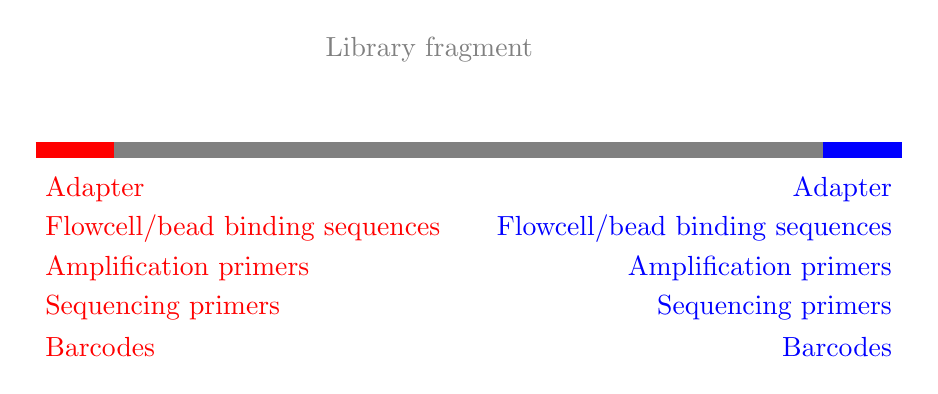
\begin{tikzpicture}
\draw [red, line width=0.2cm] (0cm,0cm) --  (1cm,0cm);
\draw [gray, line width=0.2cm] (1cm,0cm) --  (10cm,0cm);
\draw [blue, line width=0.2cm] (10cm,0cm) --  (11cm,0cm);
\node [color=red,anchor=west] at (0cm,-0.5cm){Adapter};
\node [color=blue,anchor=east] at (11cm,-0.5cm){Adapter};

\node [color=gray,anchor=south] at (5cm,1cm) {Library fragment};

\node [color=red,anchor=west] at (0cm,-1cm) {Flowcell/bead binding sequences};
\node [color=red,anchor=west] at (0cm,-1.5cm) {Amplification primers};
\node [color=red,anchor=west] at (0cm,-2cm) {Sequencing primers};      
\node [color=red,anchor=west] at (0cm,-2.5cm) {Barcodes};


\node [color=blue,anchor=east] at (11cm,-1cm) {Flowcell/bead binding sequences};
\node [color=blue,anchor=east] at (11cm,-1.5cm) {Amplification primers};
\node [color=blue,anchor=east] at (11cm,-2cm) {Sequencing primers};    
\node [color=blue,anchor=east] at (11cm,-2.5cm) {Barcodes};



\end{tikzpicture}
}
\end{figure}
\end{center}
\end{frame}

\begin{frame}[label=sec-1-1-4]{Single- or paired-end sequencing, read length - why does it matter}
\begin{center}

\begin{figure}[htb]
\setlength{\belowcaptionskip}{-1cm}
\scalebox{1}{
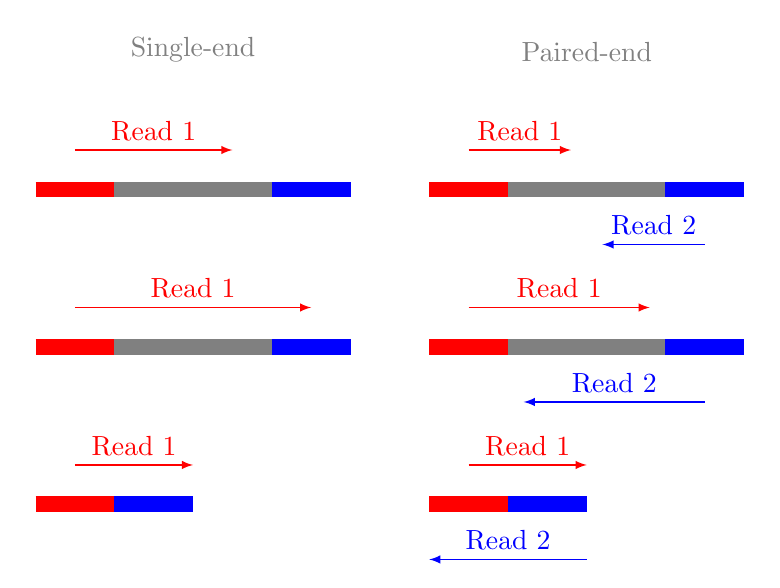
\begin{tikzpicture}

\node [color=gray,anchor=south] at (2cm,1.5cm) {Single-end};
\node [color=gray,anchor=south] at (7cm,1.5cm) {Paired-end};

\draw [red, line width=0.2cm] (0cm,0cm) --  (1cm,0cm);
\draw [gray, line width=0.2cm] (1cm,0cm) --  (3cm,0cm);
\draw [blue, line width=0.2cm] (3cm,0cm) --  (4cm,0cm);
\draw [red,-latex] (0.5cm,0.5cm) -- node [above,color=red] {Read 1} (2.5cm,0.5cm);

\begin{scope}[yshift=-2cm]
\draw [red, line width=0.2cm] (0cm,0cm) --  (1cm,0cm);
\draw [gray, line width=0.2cm] (1cm,0cm) --  (3cm,0cm);
\draw [blue, line width=0.2cm] (3cm,0cm) --  (4cm,0cm);
\draw [red,-latex] (0.5cm,0.5cm) -- node [above,color=red] {Read 1} (3.5cm,0.5cm);
\end{scope}

\begin{scope}[yshift=-4cm]
\draw [red, line width=0.2cm] (0cm,0cm) --  (1cm,0cm);
\draw [blue, line width=0.2cm] (1cm,0cm) --  (2cm,0cm);
\draw [red,-latex] (0.5cm,0.5cm) -- node [above,color=red] {Read 1} (2cm,0.5cm);
\end{scope}

\begin{scope}[xshift=5cm]
\draw [red, line width=0.2cm] (0cm,0cm) --  (1cm,0cm);
\draw [gray, line width=0.2cm] (1cm,0cm) --  (3cm,0cm);
\draw [blue, line width=0.2cm] (3cm,0cm) --  (4cm,0cm);
\draw [red,-latex] (0.5cm,0.5cm) -- node [above,color=red] {Read 1} (1.8cm,0.5cm);
\draw [blue,latex-] (2.2cm,-0.7cm) -- node [above,color=blue] {Read 2} (3.5cm,-0.7cm);
\end{scope}

\begin{scope}[yshift=-2cm,xshift=5cm]
\draw [red, line width=0.2cm] (0cm,0cm) --  (1cm,0cm);
\draw [gray, line width=0.2cm] (1cm,0cm) --  (3cm,0cm);
\draw [blue, line width=0.2cm] (3cm,0cm) --  (4cm,0cm);
\draw [red,-latex] (0.5cm,0.5cm) -- node [above,color=red] {Read 1} (2.8cm,0.5cm);
\draw [blue,latex-] (1.2cm,-0.7cm) -- node [above,color=blue] {Read 2} (3.5cm,-0.7cm);
\end{scope}

\begin{scope}[yshift=-4cm,xshift=5cm]
\draw [red, line width=0.2cm] (0cm,0cm) --  (1cm,0cm);
\draw [blue, line width=0.2cm] (1cm,0cm) --  (2cm,0cm);
\draw [red,-latex] (0.5cm,0.5cm) -- node [above,color=red] {Read 1} (2cm,0.5cm);
\draw [blue,latex-] (0cm,-0.7cm) -- node [above,color=blue] {Read 2} (2cm,-0.7cm);
\end{scope}



\end{tikzpicture}
}
\end{figure}
\end{center}
\end{frame}

\begin{frame}[label=sec-1-1-5]{Expected read lengths and sequencing qualities for common sequencing platforms}
\begin{small}

\begin{center}
\begin{tabular}{l r r l}
\alert{Platform} & \alert{Max. length} & \alert{Reads/run} & \alert{Consideration} & \\
\hline
Illumina & 2x150 & 5 billion &  & \\
HiSeq series &  &  &  & \\
\hline
Illumina & 2x300 & 25 million &  & \\
MiSeq series &  &  &  & \\
\hline
Illumina &  &  &  & \\
NextSeq series & 2x150 & 400 million &  & \\
\hline
Roche 454 & 700 & 0.7 million & High error rate & \\
GS FLX+/FLX &  &  &  & \\
\hline
Ion  PGM    318 chip & 200-400 & 4-5.5   million &  & \\
\hline
PacBio RSII & 14,000 & 0.47 million & High error rate & \\
\hline
SoliD & 2x100 & 266 million & Low error rate & \\
5500xl W &  &  & Color-space & \\
 &  &  &  & \\
\end{tabular}
\end{center}

\end{small}
\end{frame}


\section{Primary analysis}
\label{sec-2}
\subsection{Primary analysis}
\label{sec-2-1}
\begin{frame}[label=sec-2-1-1]{Primary analysis}
\begin{itemize}
\item Demultiplexing
\item Adapter trimming
\item Quality control
\end{itemize}
\end{frame}



\begin{frame}[label=sec-2-1-2]{Demultiplexing of pooled samples (if barcoded inline)}
\textcolor{blue}{AATTA}\textcolor{green}{NNNNNNNNNNNNNNN}\textcolor{white}{XXXXX}\textcolor{blue}{File 1}\\
\textcolor{white}{}\\
\textcolor{red}{AGTCG}\textcolor{green}{NNNNNNNNNNNNNNN}\textcolor{white}{XXXXX}\textcolor{red}{File 2}\\
\textcolor{white}{}\\
\textcolor{red}{AGTCG}\textcolor{green}{NNNNNNNNNNNNNNN}\textcolor{white}{XXXXX}\textcolor{red}{File 2}\\
\textcolor{white}{}\\
\textcolor{orange}{GCCAT}\textcolor{green}{NNNNNNNNNNNNNNN}\textcolor{white}{XXXXX}\textcolor{orange}{File 3}\\
\textcolor{white}{}\\
\textcolor{blue}{AATTA}\textcolor{green}{NNNNNNNNNNNNNNN}\textcolor{white}{XXXXX}\textcolor{blue}{File 1}\\
\textcolor{white}{}\\
\textcolor{orange}{GCCAT}\textcolor{green}{NNNNNNNNNNNNNNN}\textcolor{white}{XXXXX}\textcolor{orange}{File 3}\\
\textcolor{white}{}\\
\textcolor{red}{AGTCG}\textcolor{green}{NNNNNNNNNNNNNNN}\textcolor{white}{XXXXX}\textcolor{red}{File 2}\\
\end{frame}

\begin{frame}[label=sec-2-1-3]{Trimmig: Adapter removal}
Mostly \textcolor{blue}{3'adapters} disturb assembly and alignment
\textcolor{white}{dd}\\
\textcolor{white}{dd}\\
\textcolor{red}{GATTTGGGGTTCAA}NNNNNNN\textcolor{blue}{ATTAGTATCGAT}\\
\textcolor{white}{}\\
\textcolor{red}{GATTTGGGGTTCAA}NNNNNNN\textcolor{blue}{ATTAGTATCGAT}\\
\textcolor{white}{}\\
\textcolor{red}{TTGGGGTTCAA}NNNNNNN\textcolor{blue}{ATTAGTATCGAT}\\
\textcolor{white}{}\\
\textcolor{red}{GATTTGGGGTTCAA}NNNNNNN\textcolor{blue}{ATTAGTATCGAT}\\
\textcolor{white}{}\\
\textcolor{red}{ATTTGGGGTTCAA}NNNNNNN\textcolor{blue}{ATTAGTATCGAT}\\
\textcolor{white}{}\\
\textcolor{red}{GATTTGGGGTTCAA}NNNNNNN\textcolor{blue}{ATTAGTATCGAT}\\
\textcolor{white}{}\\
\end{frame}



\begin{frame}[fragile,label=sec-2-1-4]{Fastq file - 4 lines for each read}
 \begin{minted}[]{sh}
@HWI-ST141_0365:2:1101:2983:2114#TTAGGC/1
GATTTGGGGTTCAAATTAGTATCGATCAAATAGTAAATCCATTTGTTCAACTC
+
!''*((((***+))%%%++)(%%%%).1***-+*''))**55CCF>>>>>>CC
\end{minted}

\begin{enumerate}
\item sequence id (specifications can differ slightly between sequencing platforms)
\begin{itemize}
\item =@=instrument name : flowcell lane : tile number: flowcell x coordinate : flowcell y coordinates : \#barcode sequence: pair number for paired-end sequencing
\end{itemize}
\item sequence
\item + optionally followed by sequence identifier again
\item quality scores
\end{enumerate}
\end{frame}



\begin{frame}[label=sec-2-1-5]{Trimmig of low-quality bases}
\begin{itemize}
\item Trim bases with a Phred quality score <20
\item \(Quality=-10*log_{10}{P}\)

\begin{center}
\begin{tabular}{rll}
Phred Score & Probability of incorrect base & Base call accuracy\\
\hline
10 & 1 in 10 & 90\%\\
20 & 1 in 100 & 99\%\\
30 & 1 in 1000 & 99.9\%\\
\end{tabular}
\end{center}
\end{itemize}
\end{frame}


\begin{frame}[fragile,label=sec-2-1-6]{Fastq file contains both sequence reads and base quality scores}
 \alert{Fastq file}

\begin{minted}[]{sh}
@SEQ_ID
GATTTGGGGTTCAAATTAGTATCGATCAAATAGTAAATCCATTTGTTCAACTC
+
!''*((((***+))%%%++)(%%%%).1***-+*''))**55CCF>>>>>>CC
\end{minted}


\alert{Fasta file}

\begin{minted}[]{sh}
>SEQ_ID
GATTTGGGGTTCAAATTAGTATCGATCAAATAGTAAATCCATTTGTTCAACTC
\end{minted}
\end{frame}


\begin{frame}[label=sec-2-1-7]{Base qualities are encoded in ascii format}
ASCII stands for American Standard Code for Information
Interchange. An ASCII code is the numerical representation for a
character.
\begin{figure}[htb]
\centering
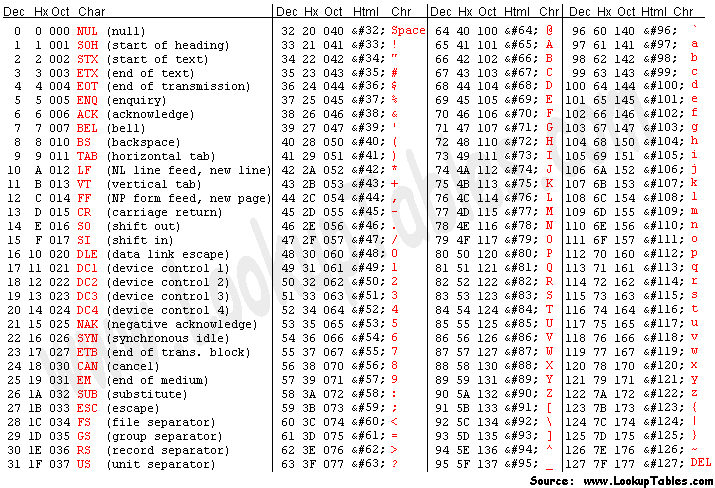
\includegraphics[width=9.5cm]{asciifull.png}
\caption{ASCII table}
\end{figure}
\end{frame}




\begin{frame}[label=sec-2-1-8]{Base qualities are encoded in ascii format}
ASCII stands for American Standard Code for Information
Interchange. An ASCII code is the numerical representation for a
character.
\begin{figure}[htb]
\centering
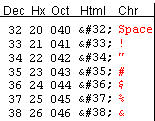
\includegraphics[width=9cm]{asciifullzoomed.png}
\caption{ASCII table}
\end{figure}
\end{frame}



\begin{frame}[label=sec-2-1-9]{ASCII encodings of sequencing platforms}
\begin{figure}[htb]
\centering
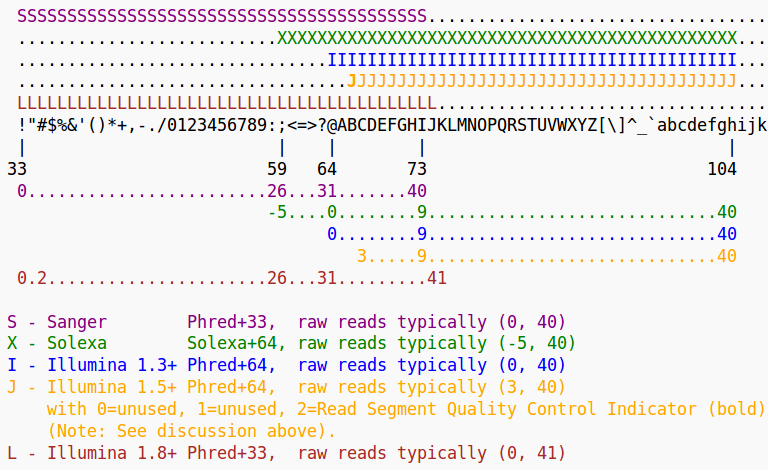
\includegraphics[width=10.5cm]{Fastq.png}
\caption{Quality score encodings}
\end{figure}
\end{frame}








\begin{frame}[label=sec-2-1-10]{Quality control tool: \href{http://www.bioinformatics.babraham.ac.uk/projects/fastqc/}{FastQC}}
Informs on:
\begin{itemize}
\item Base quality
\item Duplication
\item Overrepresentation of sequences
\begin{itemize}
\item contamination?
\item adapters?
\end{itemize}
\item GC content (should be around 50\%, in Bis-Seq lower)
\end{itemize}
\end{frame}


\begin{frame}[label=sec-2-1-11]{Quality before trimming}
\begin{figure}[htb]
\centering
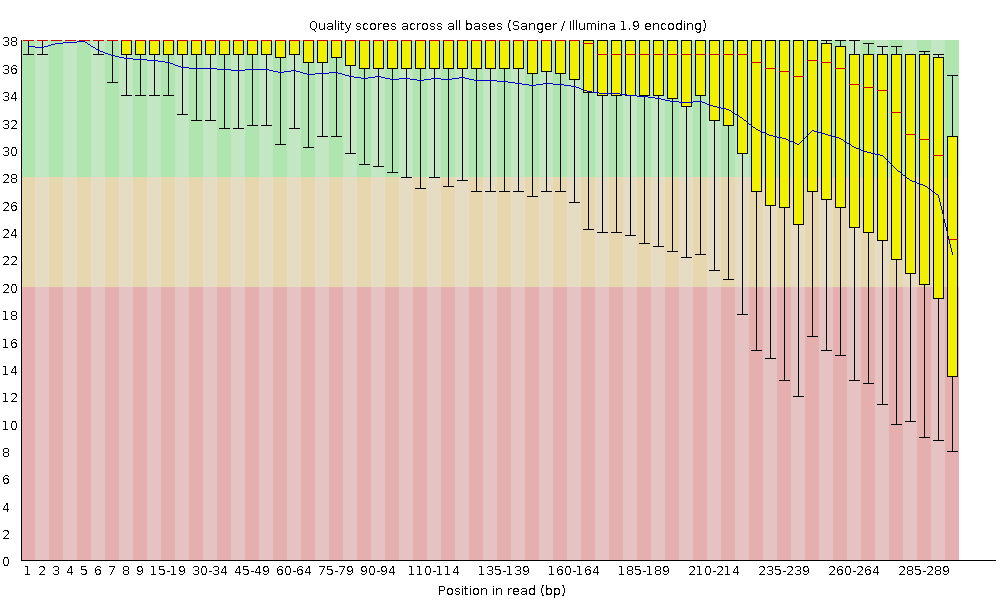
\includegraphics[width=10cm]{RawImages/per_base_quality.png}
\caption{Base-quality generally decreases with increasing sequencing length}
\end{figure}
\end{frame}

\begin{frame}[label=sec-2-1-12]{Quality after trimming}
\begin{figure}[htb]
\centering
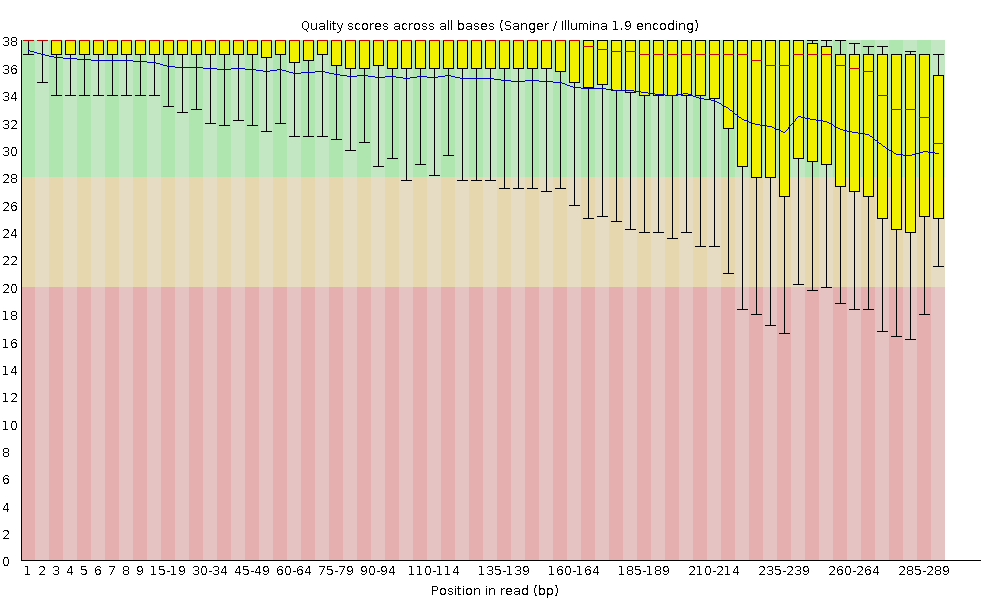
\includegraphics[width=10cm]{TrimmedImages/per_base_quality.png}
\caption{Quality after trimming}
\end{figure}
\end{frame}


\begin{frame}[label=sec-2-1-13]{Sequence bias}
For example in: 
\begin{itemize}
\item First bases of Illumina RNAseq due to 'random' hexamer primers for reverse transcription
\item RADseq fragments (cutting sites)

\begin{center}
\end{itemize}



\begin{figure}[htb]
\centering
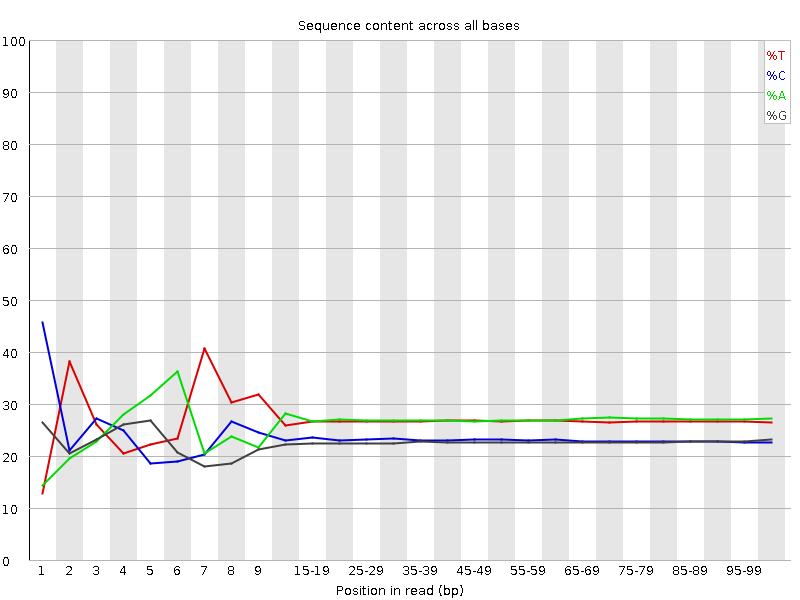
\includegraphics[width=7cm]{per_base_sequence_content.png}
\caption{Per base sequence content (FastQC output)}
\end{figure}


\tiny{\citep{Hansen2010}}
\end{center}
\end{frame}


\begin{frame}[label=sec-2-1-14]{Hexamer primers for cDNA synthesis cause sequence bias}
\definecolor{adapterp1}{rgb}{0.8431373,0.09803922,0.1098039}
\definecolor{violet}{rgb}{0.3686275,0.2352941,0.6}
\definecolor{adapterp2}{rgb}{0, 0 , 0.803922}
\definecolor{barcode1}{rgb}{0.498039,1,0}
\definecolor{barcode2}{rgb}{1, 0.647059, 0}
\definecolor{barcode4}{rgb}{0.196078, 0.803922, 0.196078}
\definecolor{sequencingprimer}{rgb}{0.9882353,0.5529412,0.3490196}
\definecolor{amplificationprimer}{rgb}{0.2705882,0.4588235,0.7058824}

\begin{center}
\begin{figure}[htb]
\setlength{\belowcaptionskip}{-1cm}
\scalebox{1}{
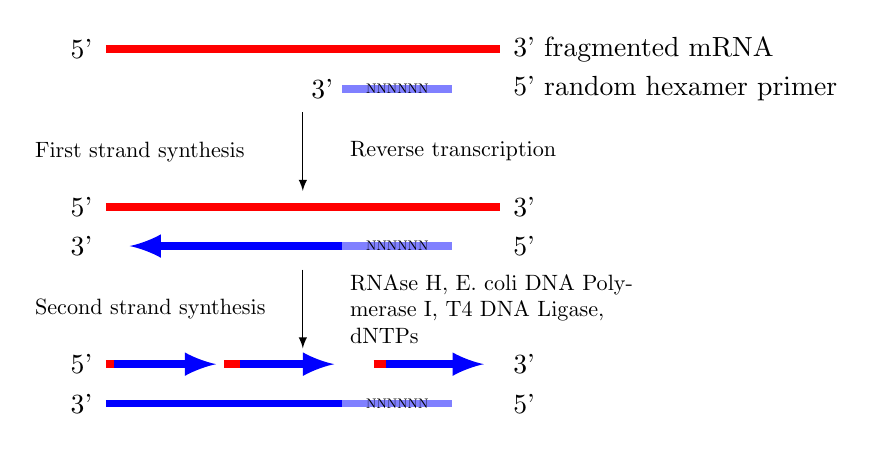
\begin{tikzpicture}
\draw [red, line width=0.1cm] (0cm,0cm) -- (5cm,0cm);
\node [anchor=east, black] at (-0.05cm,0cm) {5'};
\node [black,anchor=west] at (5.05cm,0cm) {3' fragmented mRNA};
\draw [blue!50!white, line width=0.1cm] (3cm,-0.5cm) node [black, left=-0.05cm] {3'} -- node[black,scale=0.5]{NNNNNN} (4.4cm,-0.5cm);
\node[anchor=west,black] at (5.05cm,-0.5cm) {5' random hexamer primer};

\draw [black,-latex] (2.5cm,-0.8cm) -- (2.5cm,-1.8cm);
\node [anchor=west, black, text width=4cm,scale=0.8] at (-1cm,-1.3cm) {First strand synthesis};
\node [anchor=west, black, text width=4cm,scale=0.8] at (3cm,-1.3cm) {Reverse transcription};

\draw [red, line width=0.1cm] (0cm,-2cm) -- (5cm,-2cm);
\node [anchor=east, black] at (-0.05cm,-2cm) {5'};
\node [black,anchor=west] at (5.05cm,-2cm) {3'};
\draw [blue!50!white, line width=0.1cm] (3cm,-2.5cm) -- node[black,scale=0.5]{NNNNNN} (4.4cm,-2.5cm);
\draw [blue, line width=0.1cm,latex-] (0.3cm,-2.5cm)  --  (3cm,-2.5cm);
\node [anchor=east, black] at (-0.05cm,-2.5cm) {3'};
\node [black,anchor=west] at (5.05cm,-2.5cm) {5'};


\draw [black,-latex] (2.5cm,-2.8cm) -- (2.5cm,-3.8cm);
\node [anchor=west, black, text width=4cm,scale=0.8] at (-1cm,-3.3cm) {Second strand synthesis};
\node [anchor=west, black, text width=5cm,scale=0.8] at (3cm,-3.3cm) {RNAse H, E. coli DNA Polymerase I, T4 DNA Ligase, dNTPs};



\draw [red, line width=0.1cm] (0cm,-4cm) -- (0.1cm,-4cm);
\draw [blue, line width=0.1cm,-latex] (0.1cm,-4cm) -- (1.4cm,-4cm);

\draw [red, line width=0.1cm] (1.5cm,-4cm) -- (1.7cm,-4cm);
\draw [blue, line width=0.1cm,-latex] (1.7cm,-4cm) -- (2.9cm,-4cm);

\draw [red, line width=0.1cm] (3.4cm,-4cm) -- (3.56cm,-4cm);
\draw [blue, line width=0.1cm,-latex] (3.56cm,-4cm) -- (4.8cm,-4cm);

\node [anchor=east, black] at (-0.05cm,-4cm) {5'};
\node [black,anchor=west] at (5.05cm,-4cm) {3'};

\draw [blue!50!white, line width=0.1cm] (3cm,-4.5cm) -- node[black,scale=0.5]{NNNNNN} (4.4cm,-4.5cm);
\draw [blue, line width=0.1cm] (0cm,-4.5cm)  --  (3cm,-4.5cm);
\node [anchor=east, black] at (-0.05cm,-4.5cm) {3'};
\node [black,anchor=west] at (5.05cm,-4.5cm) {5'};



\end{tikzpicture}
} 
\end{figure}
\end{center}
\end{frame}

\begin{frame}[label=sec-2-1-15]{PCR Duplicates}
Duplicates are generally removed in quantitative analyses (e.g. RNA-seq)
\begin{figure}[htb]
\centering
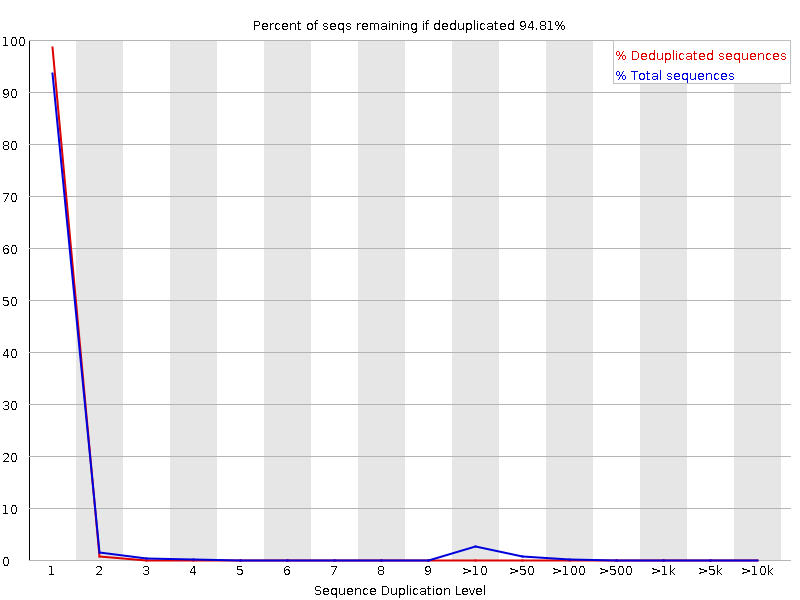
\includegraphics[width=8cm]{duplication_levels.png}
\caption{Duplication levels (FastQC output)}
\end{figure} 
\end{frame}


\section{Secondary analysis}
\label{sec-3}
\subsection{Secondary analysis}
\label{sec-3-1}
\begin{frame}[label=sec-3-1-1]{\emph{De novo} assembly}
Task: Look for overlapping regions and create contigs (contiguous sequences)
\begin{itemize}
\item Genome assembly software
\begin{itemize}
\item SOAP de NOVO
\item Velvet
\item MIRA (we use this one in the course)
\end{itemize}
\end{itemize}

\begin{itemize}
\item Transcriptome assembly software
\begin{itemize}
\item Review: \citet{Martin2011}
\item Trinity
\item MIRA
\end{itemize}
\end{itemize}
\end{frame}
\begin{frame}[label=sec-3-1-2]{\emph{De novo} assembly: Step by step}
\begin{center}
\begin{figure}[htb]
\setlength{\belowcaptionskip}{-1cm}
\scalebox{0.5}{
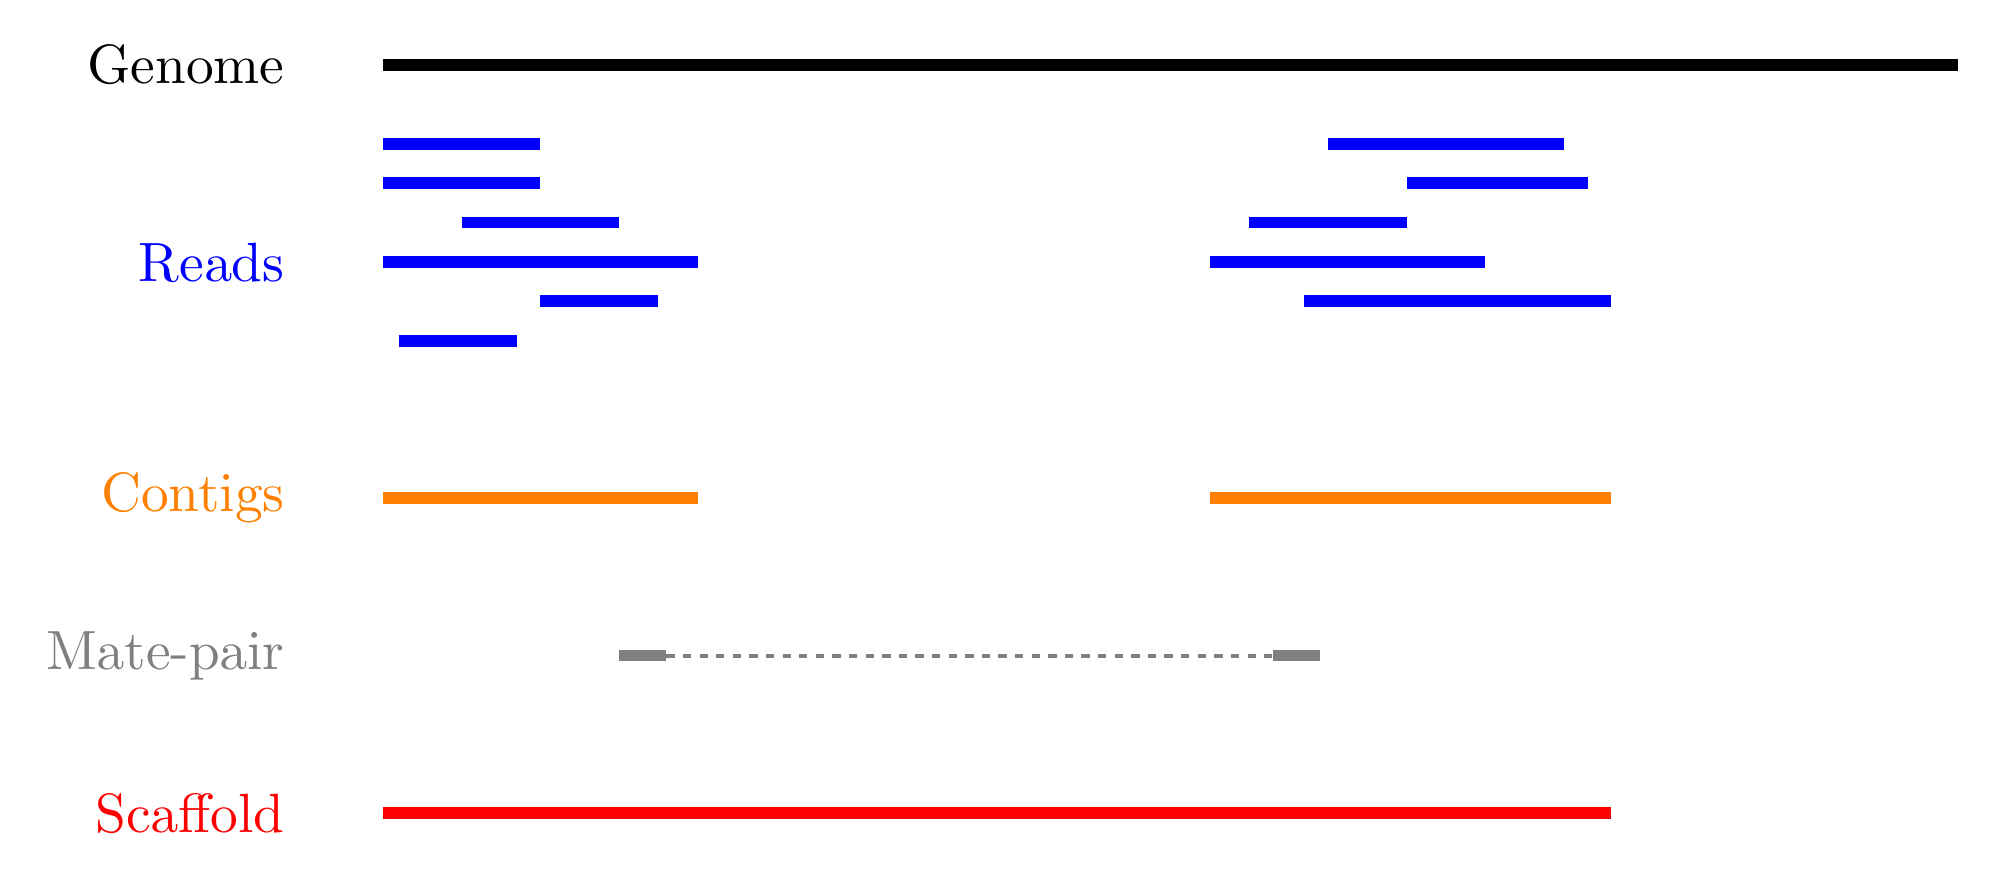
\begin{tikzpicture}

\node [anchor=east, scale=2] at (-1cm, 0.5cm) {Genome};
\node [anchor=east, scale=2,color=blue] at (-1cm, -2cm) {Reads};
\node [anchor=east, scale=2,color=orange] at (-1cm, -5cm) {Contigs};
\node [anchor=east, scale=2,color=gray] at (-1cm, -7cm) {Mate-pair};
\node [anchor=east, scale=2,color=red] at (-1cm, -9cm) {Scaffold};

\draw [line width=0.15cm, anchor=west] (0cm,0.5cm) -- (20cm,0.5cm);


\draw [line width=0.15cm, anchor=west,color=blue] (0cm,-0.5cm) -- (2cm,-0.5cm);
\draw [line width=0.15cm, anchor=west,color=blue] (0cm,-1cm) -- (2cm,-1.cm);
\draw [line width=0.15cm, anchor=west,color=blue] (1cm,-1.5cm) -- (3cm,-1.5cm);
\draw [line width=0.15cm, anchor=west,color=blue] (0cm,-2cm) -- (4cm,-2cm);
\draw [line width=0.15cm, anchor=west,color=blue] (2cm,-2.5cm) -- (3.5cm,-2.5cm);
\draw [line width=0.15cm, anchor=west,color=blue] (0.2cm,-3cm) -- (1.7cm,-3cm);

\draw [line width=0.15cm, anchor=west,color=blue] (12cm,-0.5cm) -- (15cm,-0.5cm);
\draw [line width=0.15cm, anchor=west,color=blue] (13cm,-1cm) -- (15.3cm,-1cm);
\draw [line width=0.15cm, anchor=west,color=blue] (11cm,-1.5cm) -- (13cm,-1.5cm);
\draw [line width=0.15cm, anchor=west,color=blue] (10.5cm,-2cm) -- (14cm,-2cm);
\draw [line width=0.15cm, anchor=west,color=blue] (11.7cm,-2.5cm) -- (15.6cm,-2.5cm);

\draw [line width=0.15cm, anchor=west,color=orange] (0cm,-5cm) -- (4cm,-5cm);
\draw [line width=0.15cm, anchor=west,color=orange] (10.5cm,-5cm) -- (15.6cm,-5cm);

\draw [line width=0.15cm, anchor=west,color=gray] (3cm,-7cm) -- (3.6cm,-7cm);
\draw [line width=0.05cm, dashed, anchor=west,color=gray] (3.6cm,-7cm) -- (11.3cm,-7cm);
\draw [line width=0.15cm, anchor=west,color=gray] (11.3cm,-7cm) -- (11.9cm,-7cm);

\draw [line width=0.15cm, anchor=west,color=red] (0cm,-9cm) -- (15.6cm,-9cm);

\end{tikzpicture}
} 
\end{figure}
\end{center}
\end{frame}
\begin{frame}[label=sec-3-1-3]{\emph{De novo} assembly: The N50 metric}
N50 is a single measure of the contig length size distribution in an assembly
\begin{itemize}
\item Sort contigs in descending length order
\item Size of contig above which the assembly contains at least 50\% of the
total length of all contigs
\end{itemize}

\begin{figure}[htb]
\centering
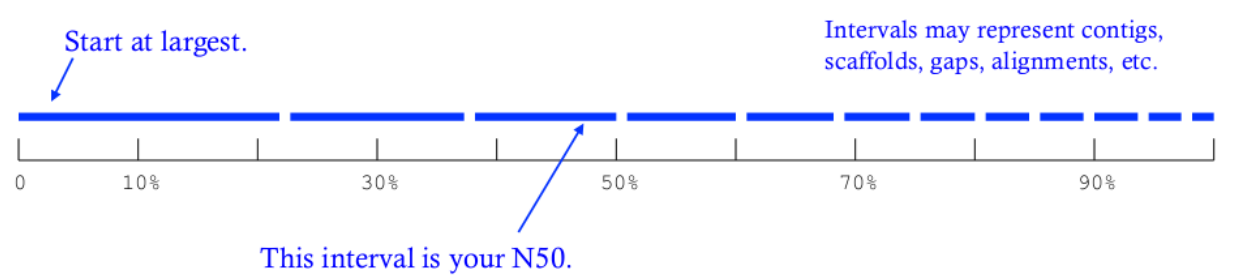
\includegraphics[width=11cm]{N50.png}
\caption{From Kane, N.C.}
\end{figure}
\end{frame}
\begin{frame}[label=sec-3-1-4]{Mapping against reference genome/transcriptome}
\begin{itemize}
\item Main purposes: 
\begin{itemize}
\item <1>Identify variants (SNPs, InDels)
\item <2>Quantify gene expression
\end{itemize}
\end{itemize}

\only<1>{
\begin{center}
\begin{figure}[htb]
\setlength{\belowcaptionskip}{-1cm}
\scalebox{0.5}{
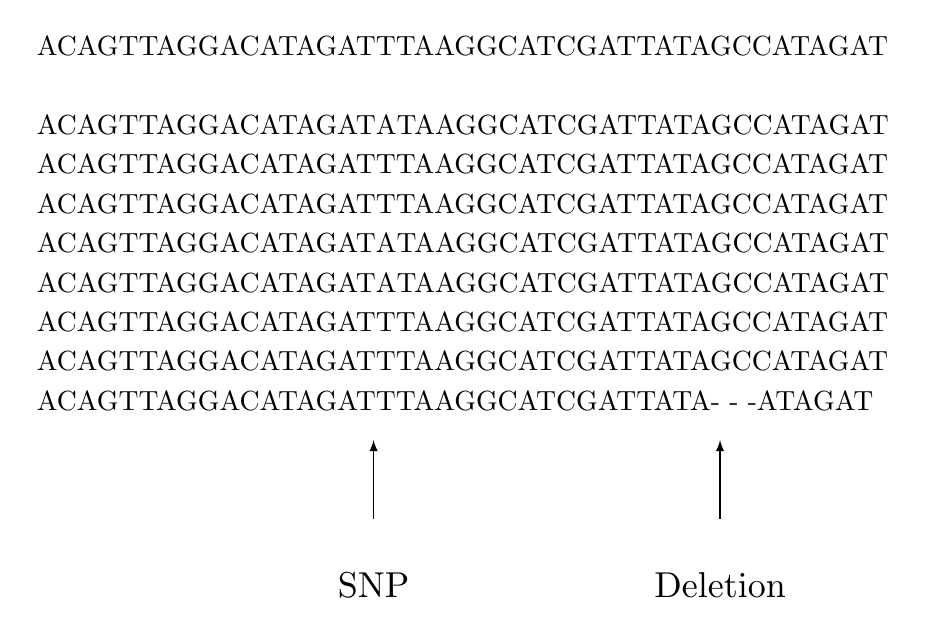
\begin{tikzpicture}
\node [anchor=west, black] at (0cm,0cm) {ACAGTTAGGACATAGATTTAAGGCATCGATTATAGCCATAGAT};
\node [anchor=west, black] at (0cm,-1cm) {ACAGTTAGGACATAGAT\alert{A}TAAGGCATCGATTATAGCCATAGAT};
\node [anchor=west, black] at (0cm,-1.5cm) {ACAGTTAGGACATAGATTTAAGGCATCGATTATAGCCATAGAT};
\node [anchor=west, black] at (0cm,-2cm) {ACAGTTAGGACATAGATTTAAGGCATCGATTATAGCCATAGAT};
\node [anchor=west, black] at (0cm,-2.5cm) {ACAGTTAGGACATAGAT\alert{A}TAAGGCATCGATTATAGCCATAGAT};
\node [anchor=west, black] at (0cm,-3cm) {ACAGTTAGGACATAGAT\alert{A}TAAGGCATCGATTATAGCCATAGAT};
\node [anchor=west, black] at (0cm,-3.5cm) {ACAGTTAGGACATAGATTTAAGGCATCGATTATAGCCATAGAT};
\node [anchor=west, black] at (0cm,-4cm) {ACAGTTAGGACATAGATTTAAGGCATCGATTATAGCCATAGAT};
\node [anchor=west, black] at (0cm,-4.5cm) {ACAGTTAGGACATAGATTTAAGGCATCGATTATA\alert{-  -  -}ATAGAT};
\draw [latex-] (4.4cm,-5cm) -- (4.4cm,-6cm) node [scale=1.3,below=0.4cm]{SNP};
\draw [latex-] (8.8cm,-5cm) -- (8.8cm,-6cm) node [scale=1.3,below=0.4cm]{Deletion};

\end{tikzpicture}
} 
\end{figure}
\end{center}
}

\only<2>{
\begin{center}
\begin{figure}[htb]
\setlength{\belowcaptionskip}{-1cm}
\scalebox{0.4}{
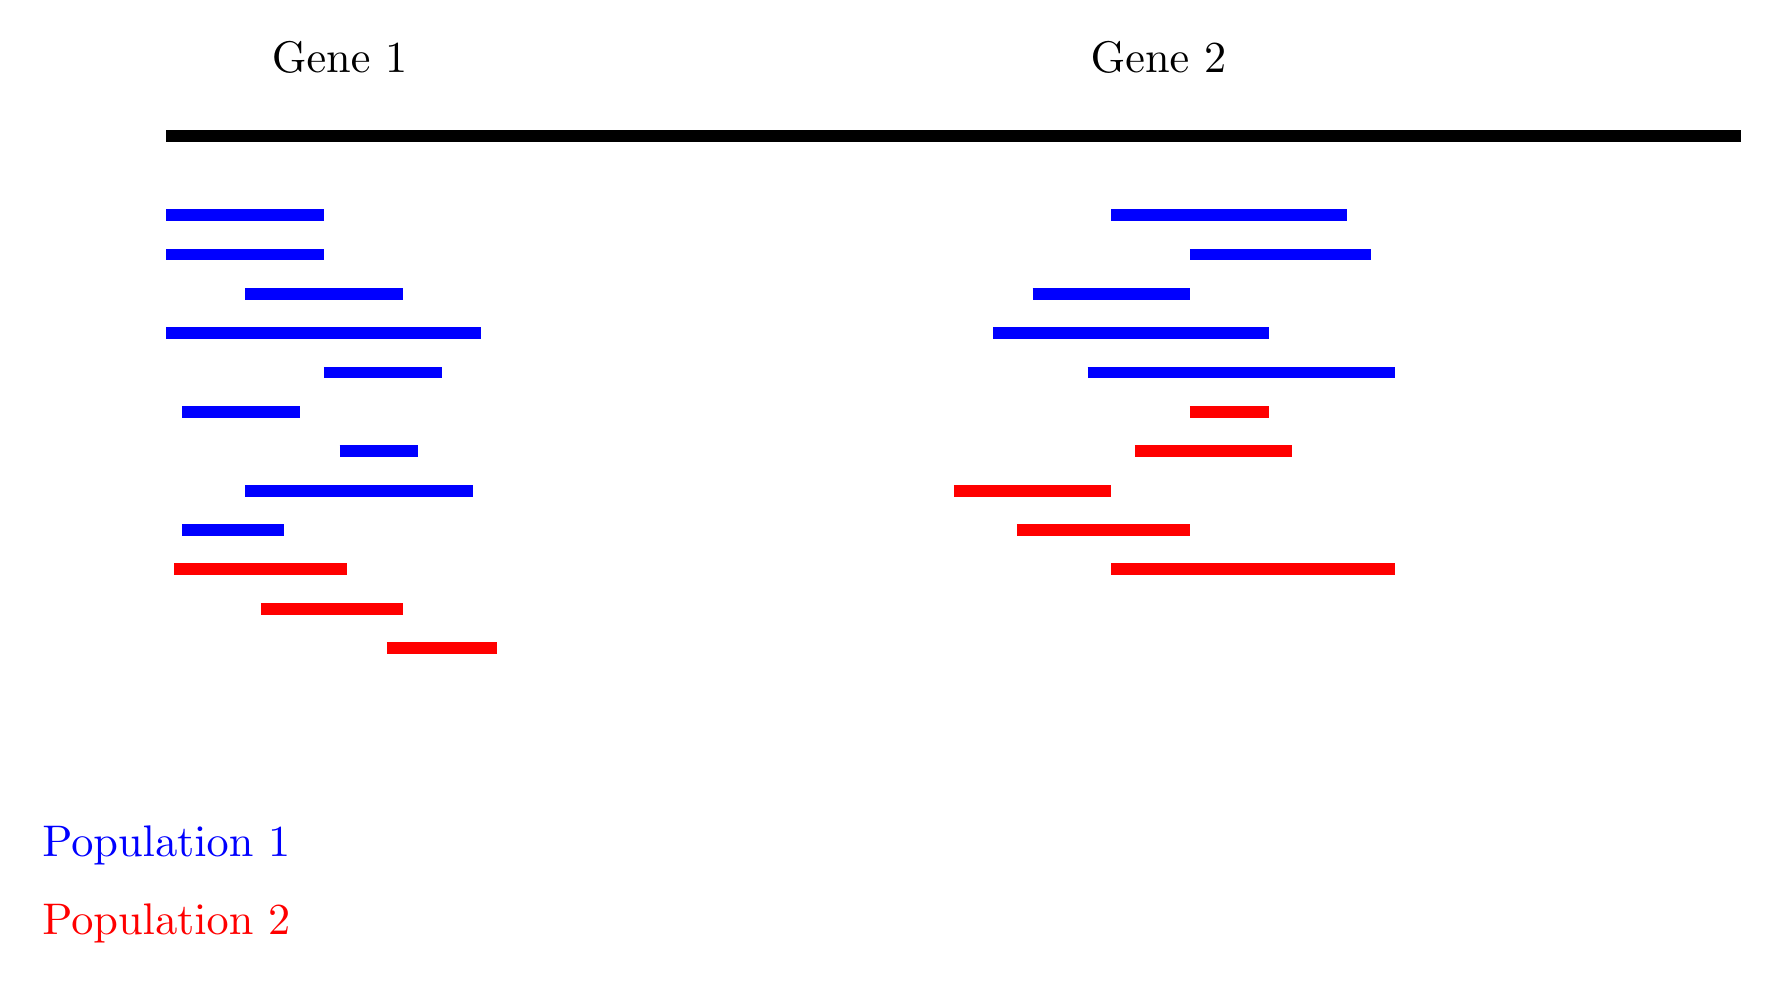
\begin{tikzpicture}

\node [scale=1.6] at (2.2cm,1.5cm) {Gene 1};
\node [scale=1.6] at (12.6cm,1.5cm) {Gene 2};


\draw [line width=0.15cm, anchor=west] (0cm,0.5cm) -- (20cm,0.5cm);


\draw [line width=0.15cm, anchor=west,color=blue] (0cm,-0.5cm) -- (2cm,-0.5cm);
\draw [line width=0.15cm, anchor=west,color=blue] (0cm,-1cm) -- (2cm,-1.cm);
\draw [line width=0.15cm, anchor=west,color=blue] (1cm,-1.5cm) -- (3cm,-1.5cm);
\draw [line width=0.15cm, anchor=west,color=blue] (0cm,-2cm) -- (4cm,-2cm);
\draw [line width=0.15cm, anchor=west,color=blue] (2cm,-2.5cm) -- (3.5cm,-2.5cm);
\draw [line width=0.15cm, anchor=west,color=blue] (0.2cm,-3cm) -- (1.7cm,-3cm);
\draw [line width=0.15cm, anchor=west,color=blue] (2.2cm,-3.5cm) -- (3.2cm,-3.5cm);
\draw [line width=0.15cm, anchor=west,color=blue] (1cm,-4cm) -- (3.9cm,-4cm);
\draw [line width=0.15cm, anchor=west,color=blue] (0.2cm,-4.5cm) -- (1.5cm,-4.5cm);
\draw [line width=0.15cm, anchor=west,color=blue] (12cm,-0.5cm) -- (15cm,-0.5cm);
\draw [line width=0.15cm, anchor=west,color=blue] (13cm,-1cm) -- (15.3cm,-1cm);
\draw [line width=0.15cm, anchor=west,color=blue] (11cm,-1.5cm) -- (13cm,-1.5cm);
\draw [line width=0.15cm, anchor=west,color=blue] (10.5cm,-2cm) -- (14cm,-2cm);
\draw [line width=0.15cm, anchor=west,color=blue] (11.7cm,-2.5cm) -- (15.6cm,-2.5cm);

\draw [line width=0.15cm, anchor=west,color=red] (0.1cm,-5cm) -- (2.3cm,-5.cm);
\draw [line width=0.15cm, anchor=west,color=red] (1.2cm,-5.5cm) -- (3cm,-5.5cm);
\draw [line width=0.15cm, anchor=west,color=red] (2.8cm,-6cm) -- (4.2cm,-6cm);
\draw [line width=0.15cm, anchor=west,color=red] (13cm,-3cm) -- (14cm,-3cm);
\draw [line width=0.15cm, anchor=west,color=red] (12.3cm,-3.5cm) -- (14.3cm,-3.5cm);
\draw [line width=0.15cm, anchor=west,color=red] (10cm,-4cm) -- (12cm,-4cm);
\draw [line width=0.15cm, anchor=west,color=red] (10.8cm,-4.5cm) -- (13cm,-4.5cm);
\draw [line width=0.15cm, anchor=west,color=red] (12cm,-5cm) -- (15.6cm,-5cm);

\node [scale=1.6,color=blue] at (0cm,-8.5cm) {Population 1};
\node [scale=1.6,color=red] at (0cm,-9.5cm) {Population 2};


\end{tikzpicture}
} 
\end{figure}
\end{center}
}
\end{frame}
\begin{frame}[label=sec-3-1-5]{Mapping: global alignment}
\begin{itemize}
\item Implemented in e.g. BWA, Bowtie2
\item Needleman-Wunsch algorithm
\item Aligns sequences in their full length
\item Used for multiple sequence alignment when sequences are similar
\end{itemize}
\begin{figure}[htb]
\centering
\includegraphics[width=8cm]{global.png}
\caption{Global alignment from \href{http://rosalind.info/glossary/local-alignment/}{rosalind.info}}
\end{figure}
\end{frame}

\begin{frame}[label=sec-3-1-6]{Mapping: local alignment}
\begin{itemize}
\item Smith-Waterman algorithm
\item Clipping of terminal unmatched bases
\item Only aligned bases contribute to the alignment's score
\item Used to target smaller portions of genes with high similarity
\begin{figure}[htb]
\centering
\includegraphics[width=8cm]{local.png}
\caption{Local alignment from \href{http://rosalind.info/glossary/local-alignment/}{rosalind.info}}
\end{figure}
\end{itemize}
\end{frame}

\begin{frame}[label=sec-3-1-7]{Splice-aware alignment of RNAseq reads to the genome}
\begin{figure}[htb]
\centering
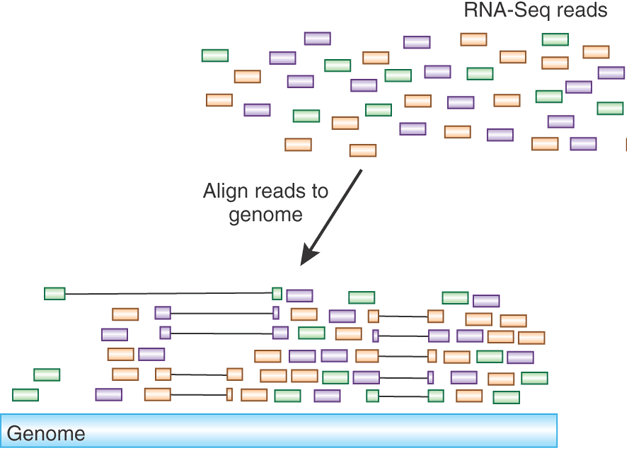
\includegraphics[width=9cm]{Haas-2010-NatureBiotechnology.png}
\caption{Adapted from \citet{Haas2010}}
\end{figure}
\end{frame}
\begin{frame}[fragile,label=sec-3-1-8]{Mapping: SAM/BAM files example}
 Output format of most alignment programs 

\begin{itemize}
\item Header lines preceded by \texttt{@}
\item One tab-delimited line per read
\end{itemize}
\begin{figure}[htb]
\centering
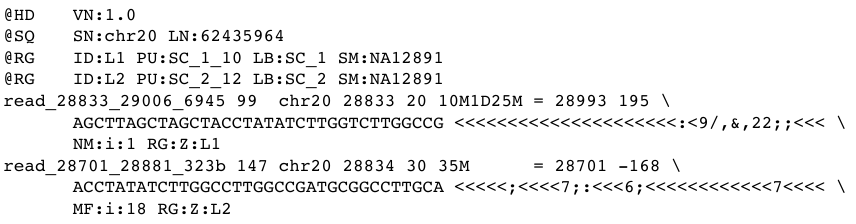
\includegraphics[width=11cm]{SAMfile.png}
\caption{Example from  \url{http://samtools.sourceforge.net/SAM1.pdf}}
\end{figure}

\begin{itemize}
\item SAM files are large
\item BAM: Compressed binary versions, not human-readable
\end{itemize}
\end{frame}

\begin{frame}[label=sec-3-1-9]{Mapping: Mandatory fields in SAM files}
\begin{center}

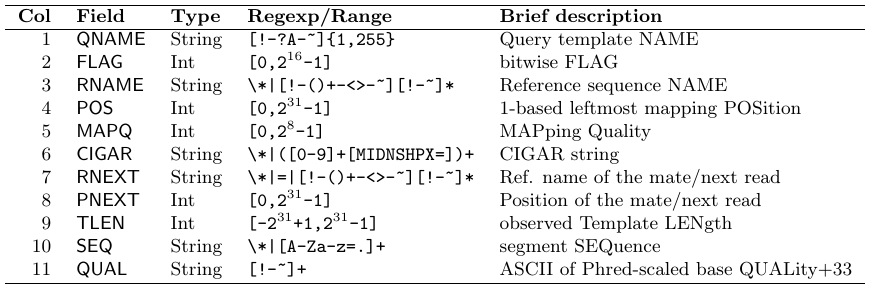
\includegraphics[width=11cm]{SamFields.png}

\normalsize{}

Explanation of the flag field (click here: \href{https://ppotato.wordpress.com/2010/08/25/samtool-bitwise-flag-paired-reads/}{Link1}, \href{http://broadinstitute.github.io/picard/explain-flags.html}{Link2})

\end{center}
\end{frame}

\begin{frame}[label=sec-3-1-10]{Mapping: Easy decoding of SAM flags}
\begin{center}

\includegraphics[width=10cm]{Flags.png}


\end{center}
\end{frame}
\begin{frame}[label=sec-3-1-11]{Mapping: CIGAR string in SAM files}
\begin{center}

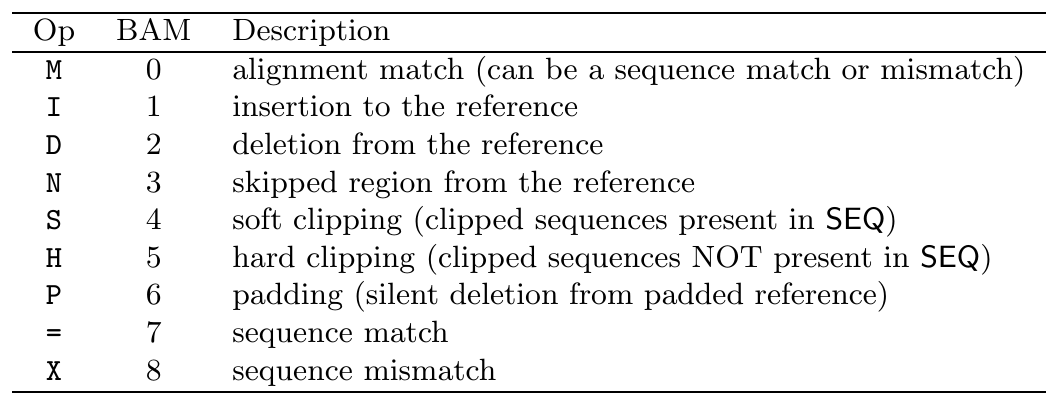
\includegraphics[width=11cm]{CIGAR.png}


\end{center}
\end{frame}
\begin{frame}[fragile,label=sec-3-1-12]{Mapping: CIGAR string example}
 \begin{minted}[]{sh}
RefPos: 1  2  3  4  5  6  7     8  9 10 11 12 13 14 15 16 
Ref:    C  C  A  T  A  C  T     G  A  A  C  T  G  A  C  T
Read:               A  C  T  A  G  A  A     T  G  G  C  T

CIGAR: 3M1I3M1D5M
\end{minted}
\end{frame}


\begin{frame}[label=sec-3-1-13]{Variant calling}
Consistent mismatches in the alignment indicate:
\begin{itemize}
\item Single Nucleotide Polymorphisms (SNPs)
\item Insertions/Deletions (InDels)
\end{itemize}
\end{frame}

\begin{frame}[label=sec-3-1-14]{VCF file format}
Variant call format
\begin{itemize}
\item described in \url{http://www.1000genomes.org/node/101}
\item informs on location and quality of each SNP
\end{itemize}
\end{frame}
\begin{frame}[label=sec-3-1-15]{VCF file information}
\begin{center}

\begin{figure}[htb]
\centering
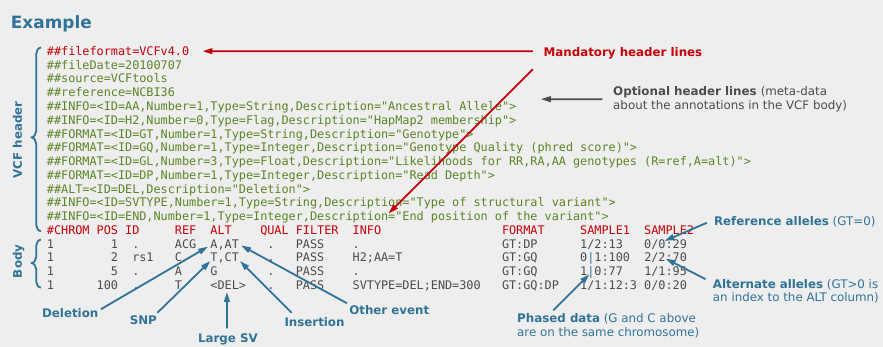
\includegraphics[width=11.5cm]{DanecekVcfFile.png}
\caption{VCF file info from \url{http://vcftools.sourceforge.net/VCF-poster.pdf}}
\end{figure}

Phased alleles are on the same chromosome strand
 \end{center}
\end{frame}

\begin{frame}[label=sec-3-1-16]{VCF file information}
\begin{center}

\begin{figure}[htb]
\centering
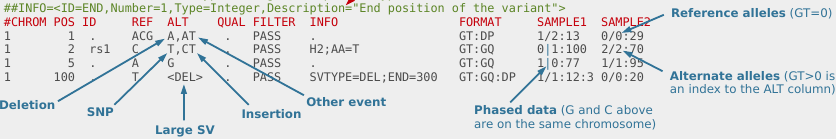
\includegraphics[width=11.5cm]{DanecekVcfFile2.png}
\caption{VCF file info from \url{http://vcftools.sourceforge.net/VCF-poster.pdf}}
\end{figure}

Phased alleles are on the same chromosome strand
 \end{center}
\end{frame}
\begin{frame}[label=sec-3-1-17]{Identified SNPs vary between programs/algorithms}
Venn diagram of the number of SNPs (coverage >400) called with four programs from the same alignment file (ddRAD tags mapped against the genome of Guppy).

\begin{center}
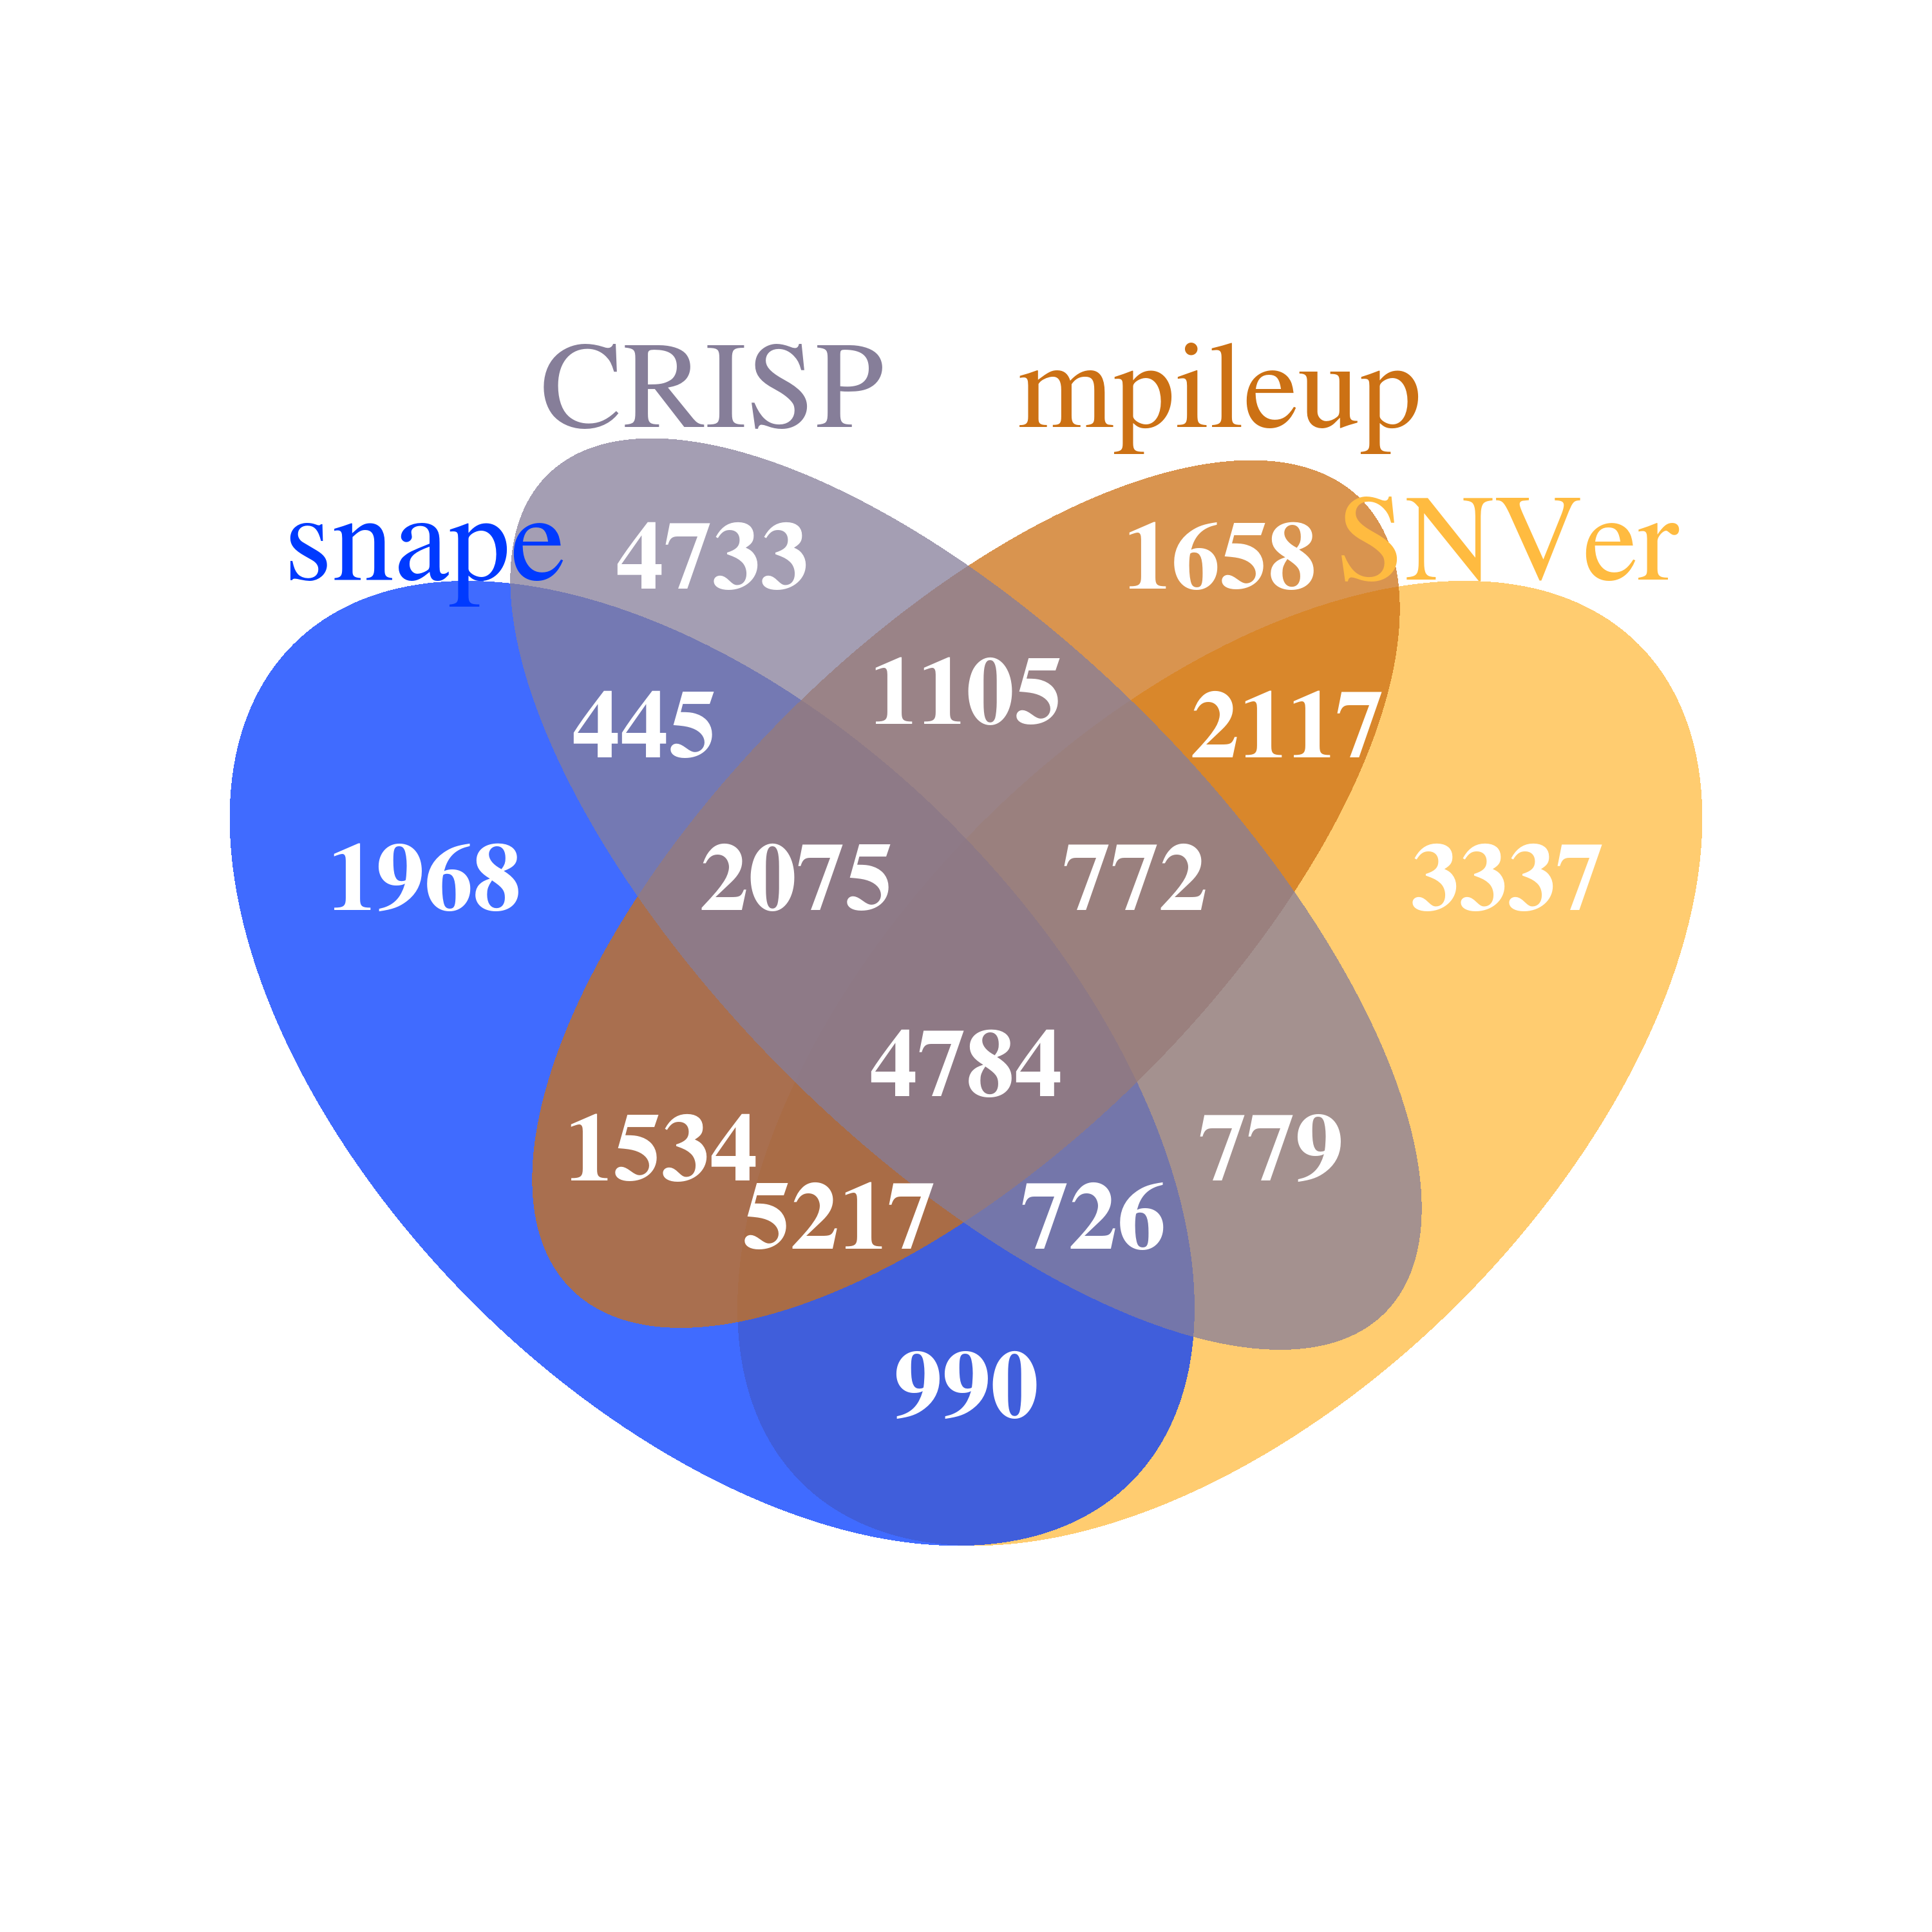
\includegraphics[width=7.5cm]{20150204_SNPs400DP.png}

\end{center}
\end{frame}
\section{Tertiary analysis}
\label{sec-4}
\subsection{Tertiary analysis}
\label{sec-4-1}
\begin{frame}[label=sec-4-1-1]{Differential gene expression analysis}

\begin{center}
\begin{figure}[htb]
\centering
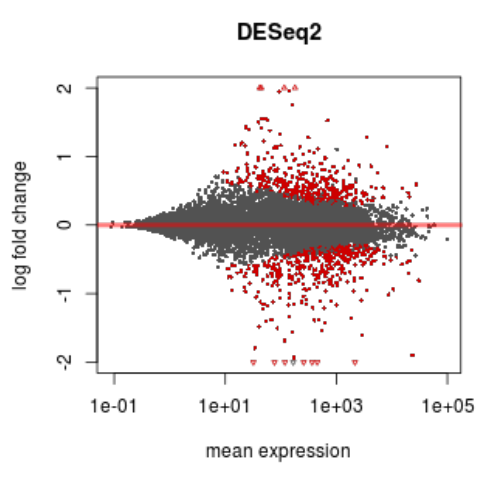
\includegraphics[width=5cm]{MAplot_DESeq2.png}
\caption{Log2 fold-change of expression over the mean of counts normalized by size factors. Differentially expressed genes (p<0.1) are red.}
\end{figure}

\tiny{From the DESeq2 R package documentation}
\end{center}
\end{frame}




\begin{frame}[label=sec-4-1-2]{Clustering}
\begin{figure}[htb]
\centering
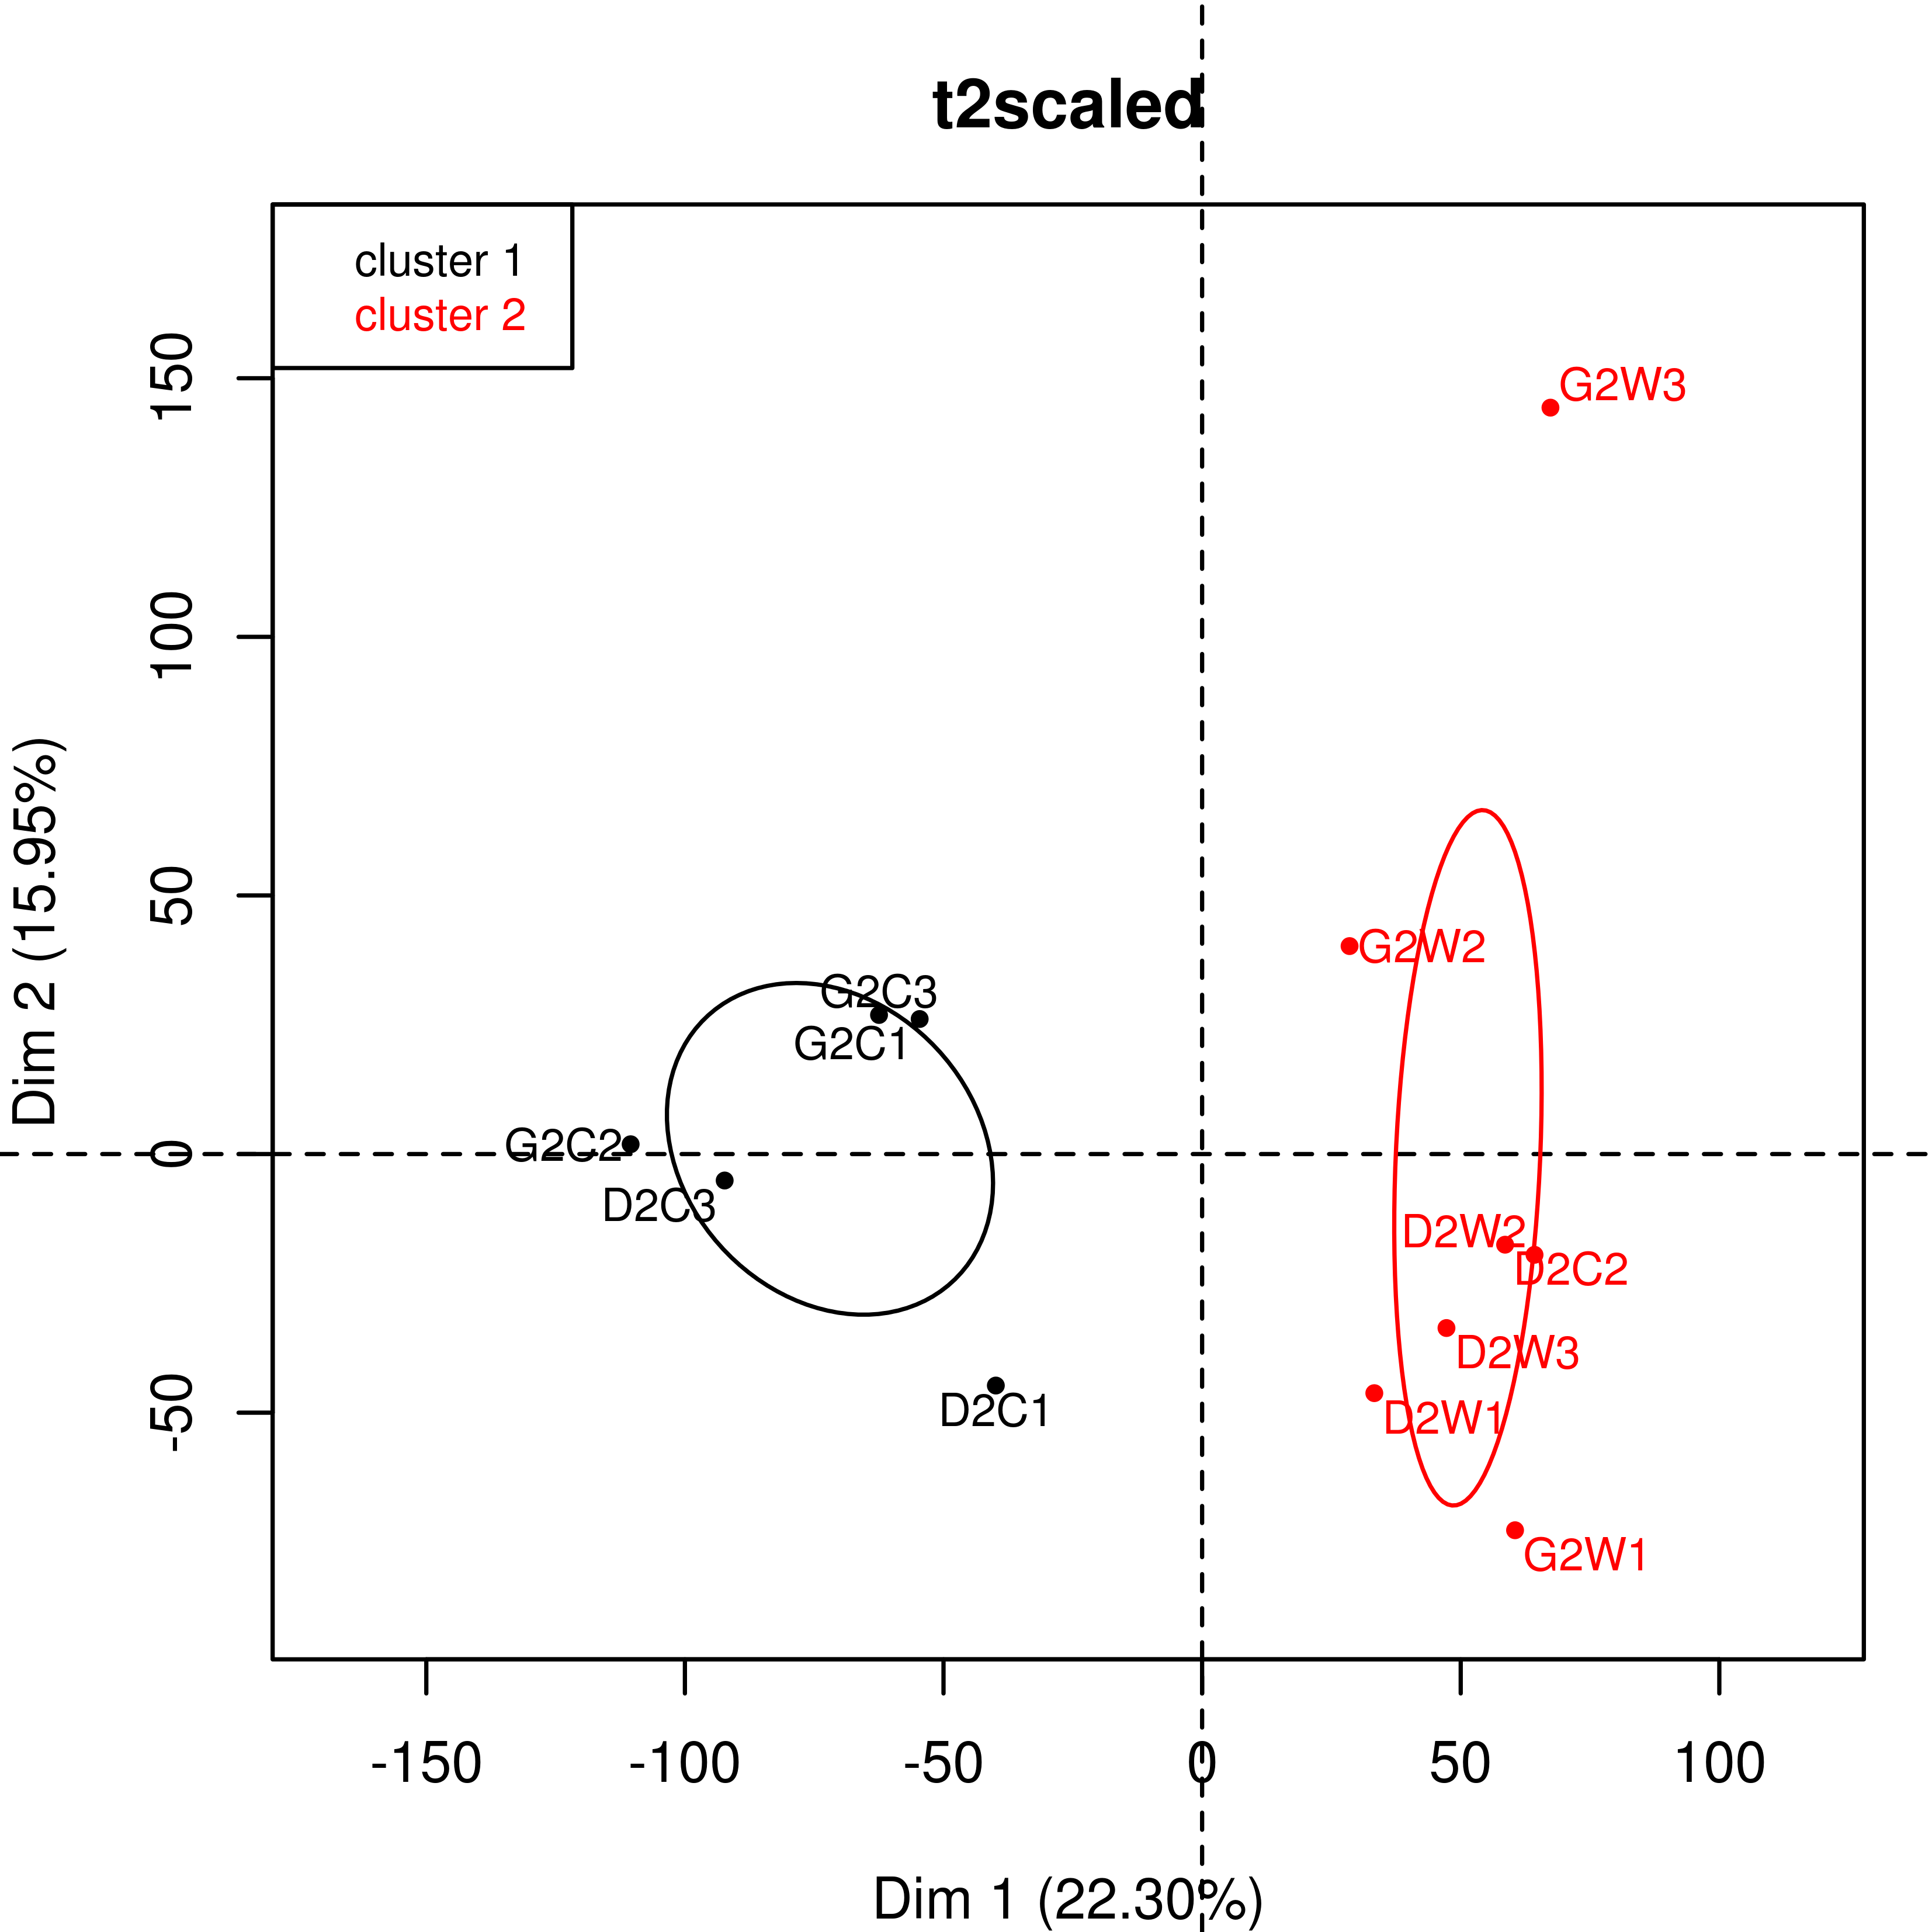
\includegraphics[width=6cm]{t2scaled_PCA.png}
\caption{Multivariate grouping of stressed (W) and control (C) seagrass samples. Most variation is explained by the first principle component}
\end{figure}
\end{frame}




\begin{frame}[label=sec-4-1-3]{Visualizing differential expression}
\begin{figure}[htb]
\centering
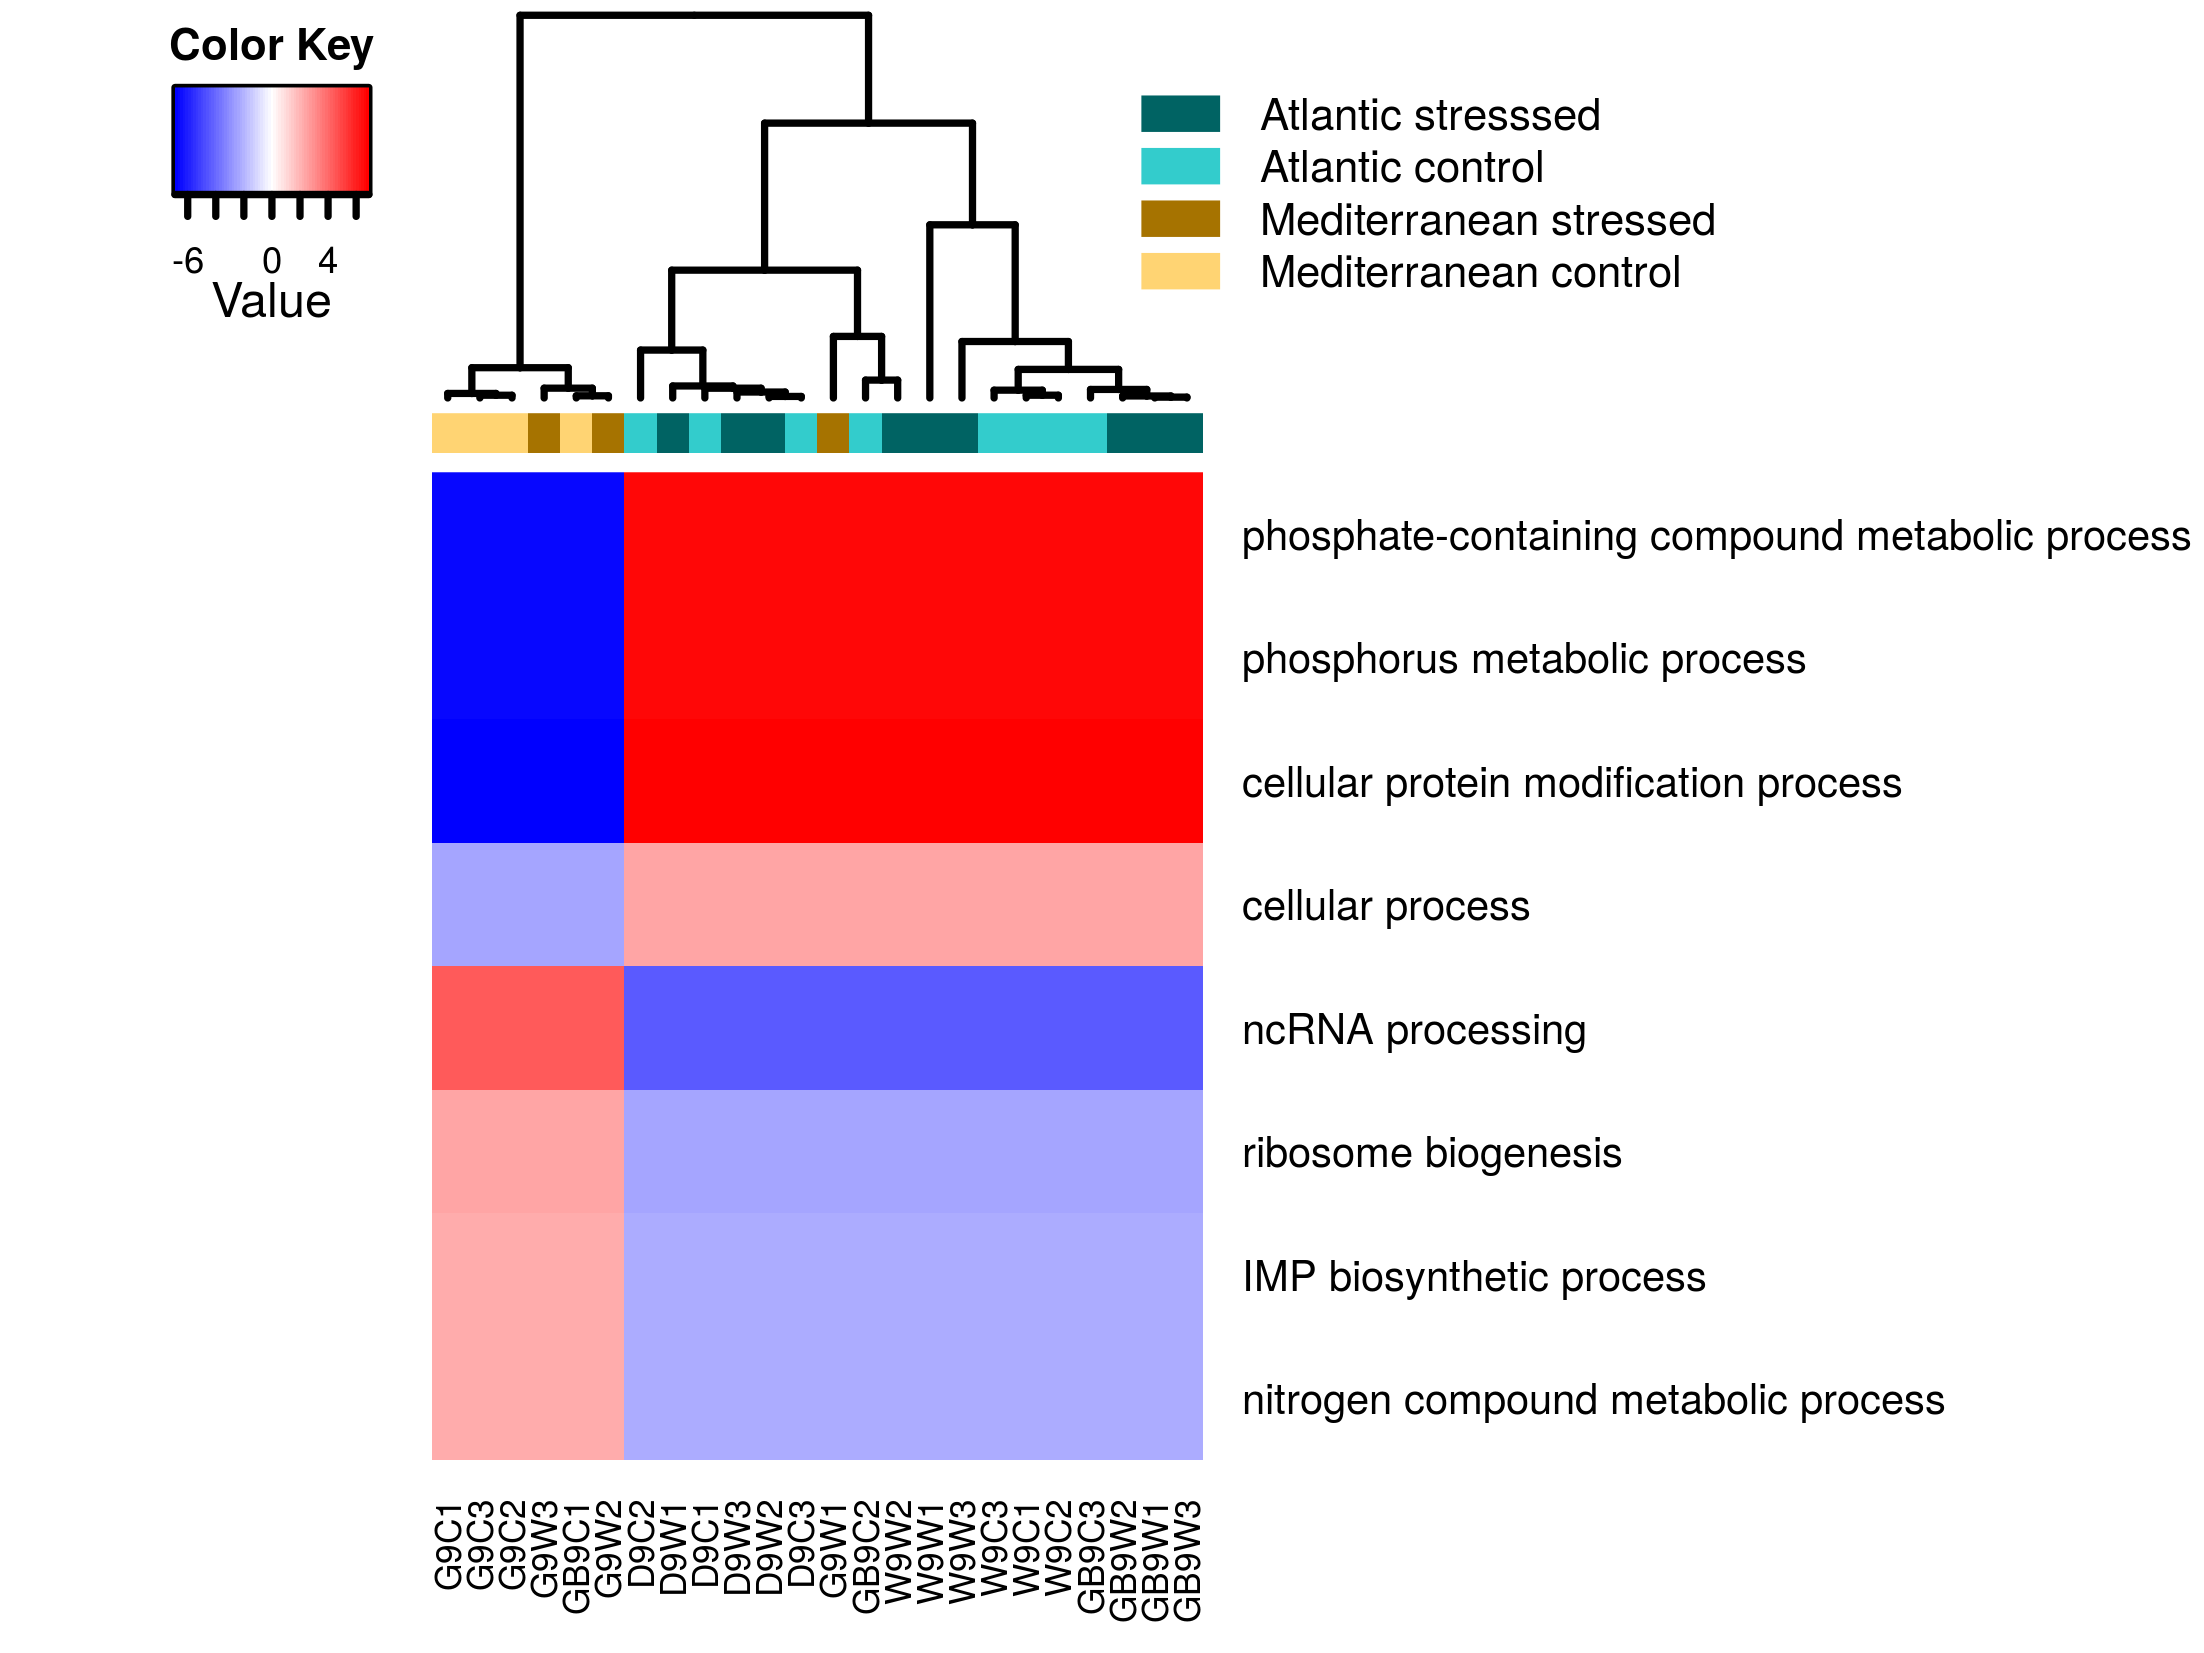
\includegraphics[width=8.5cm]{20140521_t9HeatMapCluster.png}
\caption{Heatmap of functions that were differentially expressed between Atlantic and Mediterranean seagrass samples.}
\end{figure}
\end{frame}


\begin{frame}[label=sec-4-1-4]{Outlier analysis}
\begin{center}
\begin{figure}[htb]
\setlength{\belowcaptionskip}{-1cm}
\scalebox{0.7}{
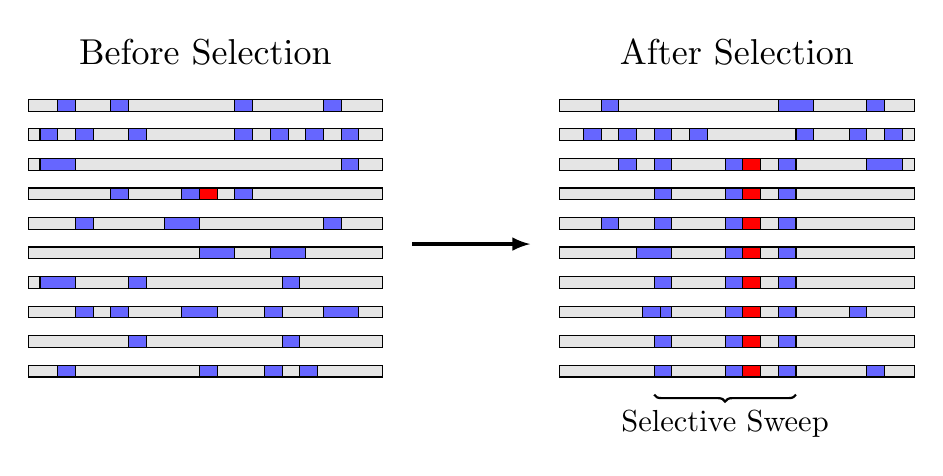
\begin{tikzpicture}[scale=1.5,decoration=brace]
\begin{scope}[scale=0.5,xshift=10cm,yshift=20cm,color=black,]
\node [scale=1.3](Before) at  (-4.5,0) {Before Selection};

\node [scale=1.3] (After) at (4.5,0) {After Selection};

\draw [fill=gray!20](-7.5,-1) rectangle (-1.5,-0.8); 
\draw [fill=blue!60] (-7,-1) rectangle (-6.7,-0.8);
\draw [fill=blue!60] (-6.1,-1) rectangle (-5.8,-0.8);
\draw [fill=blue!60] (-4,-1) rectangle (-3.7,-0.8);
\draw [fill=blue!60] (-2.5,-1) rectangle (-2.2,-0.8);

\draw [fill=gray!20](7.5,-1) rectangle (1.5,-0.8);
\draw [fill=blue!60] (7,-1) rectangle (6.7,-0.8);
\draw [fill=blue!60] (5.8,-1) rectangle (5.2,-0.8);
\draw [fill=blue!60] (2.5,-1) rectangle (2.2,-0.8);




\draw [fill=gray!20](-7.5,-1.3) rectangle (-1.5,-1.5);
\draw [fill=blue!60] (-7.3,-1.3) rectangle (-7,-1.5);
\draw [fill=blue!60] (-6.7,-1.3) rectangle (-6.4,-1.5);
\draw [fill=blue!60] (-5.8,-1.3) rectangle (-5.5,-1.5);
\draw [fill=blue!60] (-4,-1.3) rectangle (-3.7,-1.5);
\draw [fill=blue!60] (-3.4,-1.3) rectangle (-3.1,-1.5);
\draw [fill=blue!60] (-2.8,-1.3) rectangle (-2.5,-1.5);
\draw [fill=blue!60] (-2.2,-1.3) rectangle (-1.9,-1.5);



\draw [fill=gray!20](7.5,-1.3) rectangle (1.5,-1.5);
\draw [fill=blue!60] (7.3,-1.3) rectangle (7,-1.5);
\draw [fill=blue!60] (6.7,-1.3) rectangle (6.4,-1.5);
\draw [fill=blue!60] (5.8,-1.3) rectangle (5.5,-1.5);
\draw [fill=blue!60] (4,-1.3) rectangle (3.7,-1.5);
\draw [fill=blue!60] (3.4,-1.3) rectangle (3.1,-1.5);
\draw [fill=blue!60] (2.8,-1.3) rectangle (2.5,-1.5);
\draw [fill=blue!60] (2.2,-1.3) rectangle (1.9,-1.5);




\draw [fill=gray!20](-7.5,-1.8) rectangle (-1.5,-2);
\draw [fill=blue!60] (-7.3,-1.8) rectangle (-6.7,-2);
\draw [fill=blue!60] (-2.2,-1.8) rectangle (-1.9,-2);

\draw [fill=gray!20](7.5,-1.8) rectangle (1.5,-2);
\draw [fill=blue!60] (7.3,-1.8) rectangle (6.7,-2);
\draw [fill=blue!60] (5.5,-1.8) rectangle (5.2,-2);
\draw [fill=red] (4.9,-1.8) rectangle (4.6,-2);
\draw [fill=blue!60] (4.6,-1.8) rectangle (4.3,-2);
\draw [fill=blue!60] (3.4,-1.8) rectangle (3.1,-2);
\draw [fill=blue!60] (2.8,-1.8) rectangle (2.5,-2);



\draw [fill=gray!20](-7.5,-2.3) rectangle (-1.5,-2.5);

\draw [fill=blue!60] (-6.1,-2.3) rectangle (-5.8,-2.5);

\draw [fill=blue!60] (-4.9,-2.3) rectangle (-4.6,-2.5);
\draw [fill=red] (-4.6,-2.3) rectangle (-4.3,-2.5);
\draw [fill=blue!60] (-4,-2.3) rectangle (-3.7,-2.5);



\draw [fill=gray!20](7.5,-2.3) rectangle (1.5,-2.5);
\draw [fill=blue!60] (5.5,-2.3) rectangle (5.2,-2.5);
\draw [fill=red] (4.9,-2.3) rectangle (4.6,-2.5);
\draw [fill=blue!60] (4.6,-2.3) rectangle (4.3,-2.5);
\draw [fill=blue!60] (3.4,-2.3) rectangle (3.1,-2.5);


\draw [fill=gray!20](-7.5,-2.8) rectangle (-1.5,-3);
\draw [fill=blue!60] (-6.7,-2.8) rectangle (-6.4,-3);
\draw [fill=blue!60] (-5.2,-2.8) rectangle (-4.6,-3);
\draw [fill=blue!60] (-2.5,-2.8) rectangle (-2.2,-3);



\draw [fill=gray!20](7.5,-2.8) rectangle (1.5,-3);
\draw [fill=blue!60] (5.5,-2.8) rectangle (5.2,-3);
\draw [fill=red] (4.9,-2.8) rectangle (4.6,-3);
\draw [fill=blue!60] (4.6,-2.8) rectangle (4.3,-3);
\draw [fill=blue!60] (3.4,-2.8) rectangle (3.1,-3);
\draw [fill=blue!60] (2.5,-2.8) rectangle (2.2,-3);



\draw [fill=gray!20](-7.5,-3.3) rectangle (-1.5,-3.5);
\draw [fill=blue!60] (-4.6,-3.3) rectangle (-4,-3.5);
\draw [fill=blue!60] (-3.4,-3.3) rectangle (-2.8,-3.5);



\draw [fill=gray!20](7.5,-3.3) rectangle (1.5,-3.5);
\draw [fill=blue!60] (5.5,-3.3) rectangle (5.2,-3.5);
\draw [fill=red] (4.9,-3.3) rectangle (4.6,-3.5);
\draw [fill=blue!60] (4.6,-3.3) rectangle (4.3,-3.5);
\draw [fill=blue!60] (3.4,-3.3) rectangle (3.1,-3.5);
\draw [fill=blue!60] (3.4,-3.3) rectangle (2.8,-3.5);



\draw [fill=gray!20](-7.5,-3.8) rectangle (-1.5,-4);
\draw [fill=blue!60] (-7.3,-3.8) rectangle (-6.7,-4);
\draw [fill=blue!60] (-5.8,-3.8) rectangle (-5.5,-4);
\draw [fill=blue!60] (-3.2,-3.8) rectangle (-2.9,-4);

\draw [fill=gray!20](7.5,-3.8) rectangle (1.5,-4);
\draw [fill=blue!60] (5.5,-3.8) rectangle (5.2,-4);
\draw [fill=red] (4.9,-3.8) rectangle (4.6,-4);
\draw [fill=blue!60] (4.6,-3.8) rectangle (4.3,-4);
\draw [fill=blue!60] (3.4,-3.8) rectangle (3.1,-4);



\draw [fill=gray!20](-7.5,-4.3) rectangle (-1.5,-4.5);
\draw [fill=blue!60] (-6.7,-4.3) rectangle (-6.4,-4.5);
\draw [fill=blue!60] (-6.1,-4.3) rectangle (-5.8,-4.5);
\draw [fill=blue!60] (-4.9,-4.3) rectangle (-4.3,-4.5);
\draw [fill=blue!60] (-3.5,-4.3) rectangle (-3.2,-4.5);
\draw [fill=blue!60] (-2.5,-4.3) rectangle (-1.9,-4.5);


\draw [fill=gray!20](7.5,-4.3) rectangle (1.5,-4.5);
\draw [fill=blue!60] (6.7,-4.3) rectangle (6.4,-4.5);
\draw [fill=blue!60] (5.5,-4.3) rectangle (5.2,-4.5);
\draw [fill=red] (4.9,-4.3) rectangle (4.6,-4.5);
\draw [fill=blue!60] (4.6,-4.3) rectangle (4.3,-4.5);
\draw [fill=blue!60] (3.4,-4.3) rectangle (3.1,-4.5);
\draw [fill=blue!60] (3.2,-4.3) rectangle (2.9,-4.5);



\draw [fill=gray!20](-7.5,-4.8) rectangle (-1.5,-5);
\draw [fill=blue!60] (-5.8,-4.8) rectangle (-5.5,-5);
\draw [fill=blue!60] (-3.2,-4.8) rectangle (-2.9,-5);

\draw [fill=gray!20](7.5,-4.8) rectangle (1.5,-5);
\draw [fill=blue!60] (5.5,-4.8) rectangle (5.2,-5);
\draw [fill=red] (4.9,-4.8) rectangle (4.6,-5);
\draw [fill=blue!60] (4.6,-4.8) rectangle (4.3,-5);
\draw [fill=blue!60] (3.4,-4.8) rectangle (3.1,-5);



\draw [fill=gray!20](-7.5,-5.3) rectangle (-1.5,-5.5);
\draw [fill=blue!60] (-7,-5.3) rectangle (-6.7,-5.5);
\draw [fill=blue!60] (-4.6,-5.3) rectangle (-4.3,-5.5);
\draw [fill=blue!60] (-3.5,-5.3) rectangle (-3.2,-5.5);
\draw [fill=blue!60] (-2.9,-5.3) rectangle (-2.6,-5.5);

\draw [fill=gray!20](7.5,-5.3) rectangle (1.5,-5.5);
\draw [fill=blue!60] (7,-5.3) rectangle (6.7,-5.5);
\draw [fill=blue!60] (5.5,-5.3) rectangle (5.2,-5.5);
\draw [fill=red] (4.9,-5.3) rectangle (4.6,-5.5);
\draw [fill=blue!60] (4.6,-5.3) rectangle (4.3,-5.5);
\draw [fill=blue!60] (3.4,-5.3) rectangle (3.1,-5.5);

\draw [decorate,thick] (5.5,-5.8) -- (3.1,-5.8);
\node [scale=1.1] at (4.3,-6.3){Selective Sweep};

\draw [-latex, very thick] (-1,-3.25) -- (1,-3.25);
\end{scope}

\end{tikzpicture}
}
\end{figure}
\vspace{0.2cm}
\tiny{Based on \citet{Vitti2012}}
\end{center}
\end{frame}
\begin{frame}[label=sec-4-1-5]{Outlier detection}
\begin{center}
\begin{figure}[htb]
\setlength{\belowcaptionskip}{-1cm}
\scalebox{0.5}{
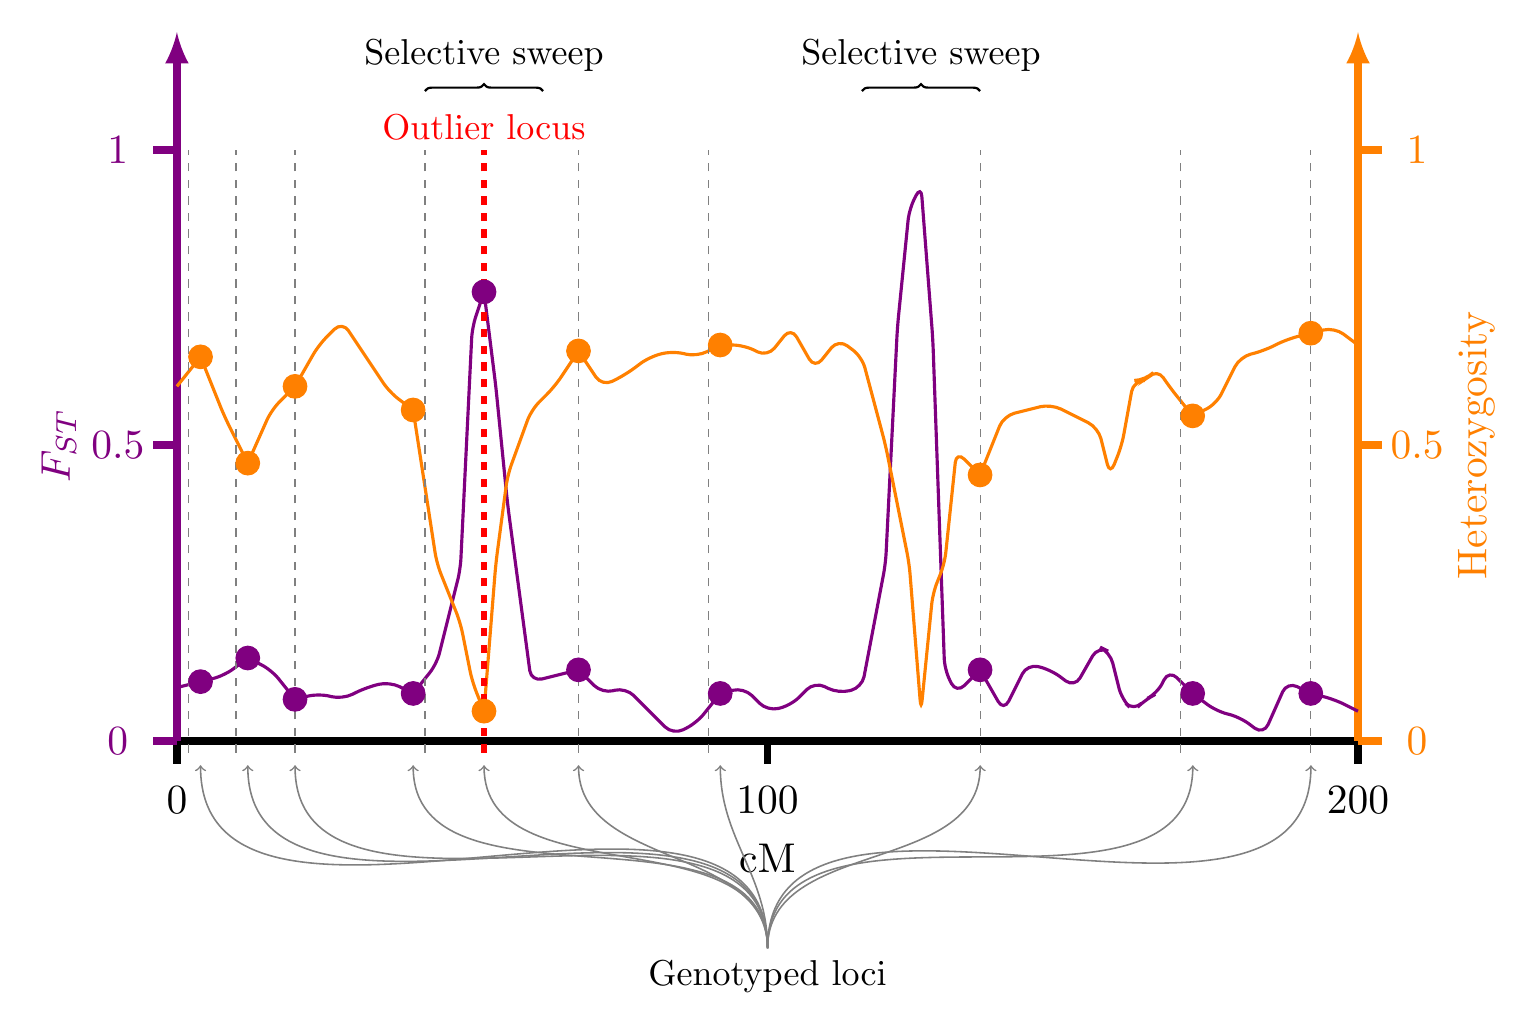
\begin{tikzpicture}[scale=1.5,decoration=brace]

\draw [line width=0.1cm] (0,0) -- (10,0);
\draw [line width=0.1cm,-latex,color=red!50!yellow] (10,0) -- (10,6);
\draw [line width=0.1cm,-latex,color=red!50!blue] (0,0) -- (0,6);
\draw [line width=0.1cm] (0,0) -- (0,-0.2);
\draw [line width=0.1cm] (5,0) -- (5,-0.2);
\draw [line width=0.1cm] (10,0) -- (10,-0.2);

\draw [line width=0.1cm,color=red!50!blue] (-0.2,0) -- (0,0);
\draw [line width=0.1cm,color=red!50!blue] (-0.2,2.5) -- (0,2.5);
\draw [line width=0.1cm,color=red!50!blue] (-0.2,5) -- (0,5);

\draw [line width=0.1cm,color=red!50!yellow] (10.2,0) -- (10,0);
\draw [line width=0.1cm,color=red!50!yellow] (10.2,2.5) -- (10,2.5);
\draw [line width=0.1cm,color=red!50!yellow] (10.2,5) -- (10,5);

\node [scale=1.5,color=black] at (5,-1) {cM};
\node [scale=1.5,color=black] at (0,-0.5) {0};
\node [scale=1.5,color=black] at (5,-0.5) {100};
\node [scale=1.5,color=black] at (10,-0.5) {200};

\node [scale=1.5,color=red!50!blue] at (-0.5,0) {0};
\node [scale=1.5,color=red!50!blue] at (-0.5,2.5) {0.5};
\node [scale=1.5,color=red!50!blue] at (-0.5,5) {1};

\node [scale=1.5,color=red!50!yellow] at (10.5,0) {0};
\node [scale=1.5,color=red!50!yellow] at (10.5,2.5) {0.5};
\node [scale=1.5,color=red!50!yellow] at (10.5,5) {1};

\node [scale=1.5,color=red!50!blue,rotate=90] at (-1,2.5) {$F_{ST}$};
\node [scale=1.5,color=red!50!yellow,rotate=90] at (11,2.5) {Heterozygosity};

% Fst values
\begin{scope}[yscale=5]
\draw [color=red!50!blue,rounded corners,line width=0.04cm] (0,0.09)--
(0.2,0.1)--
(0.4,0.11)--
(0.6,0.14)--
(0.8,0.12)--
(1,0.07)--
(1.2,0.08)--
(1.4,0.07)--
(1.6,0.09)--
(1.8,0.1)--
(2,0.08)--
(2.2,0.13)--
(2.4,0.29)--
(2.5,0.7)--
(2.6,0.76)--
(2.7,0.6)--
(2.8,0.4)--
(3,0.1)--
(3.2,0.11)--
(3.4,0.12)--
(3.6,0.08)--
(3.8,0.09)--
(4,0.05)--
(4.2,0.01)--
(4.4,0.03)--
(4.6,0.08)--
(4.8,0.09)--
(5,0.05)--
(5.2,0.06)--
(5.4,0.1)--
(5.6,0.08)--
(5.8,0.09)--
(6,0.3)--
(6.1,0.7)--
(6.2,0.9)--
(6.3,0.94)--
(6.4,0.68)--
(6.5,0.12)--
(6.6,0.08)--
(6.8,0.12)--
(7,0.05)--
(7.2,0.13)--
(7.4,0.12)--
(7.6,0.09)--
(7.8,0.16)--
(7.9,0.15)--
(8,0.07)--
(8.1,0.05)--
(8.2,0.07)--
(8.3,0.08)--
(8.4,0.12)--
(8.6,0.08)--
(8.8,0.05)--
(9,0.04)--
(9.2,0.01)--
(9.4,0.1)--
(9.6,0.08)--
(9.8,0.07)--
(10,0.05);
\end{scope}

% Heterozygosity
\begin{scope}[yscale=5]
\draw [color=red!50!yellow,rounded corners,line width=0.04cm] (0,0.6)--
(0.2,0.65)--
(0.4,0.55)--
(0.6,0.47)--
(0.8,0.56)--
(1,0.6)--
(1.2,0.67)--
(1.4,0.71)--
(1.6,0.65)--
(1.8,0.59)--
(2,0.56)--
(2.2,0.3)--
(2.4,0.2)--
(2.5,0.1)--
(2.6,0.05)--
(2.7,0.3)--
(2.8,0.45)--
(3,0.56)--
(3.2,0.6)--
(3.4,0.66)--
(3.6,0.6)--
(3.8,0.62)--
(4,0.65)--
(4.2,0.66)--
(4.4,0.65)--
(4.6,0.67)--
(4.8,0.67)--
(5,0.65)--
(5.2,0.7)--
(5.4,0.63)--
(5.6,0.68)--
(5.8,0.65)--
(6,0.5)--
(6.1,0.4)--
(6.2,0.3)--
(6.3,0.05)--
(6.4,0.25)--
(6.5,0.3)--
(6.6,0.49)--
(6.8,0.45)--
(7,0.55)--
(7.2,0.56)--
(7.4,0.57)--
(7.6,0.55)--
(7.8,0.53)--
(7.9,0.45)--
(8,0.5)--
(8.1,0.61)--
(8.2,0.61)--
(8.3,0.63)--
(8.4,0.6)--
(8.6,0.55)--
(8.8,0.57)--
(9,0.65)--
(9.2,0.66)--
(9.4,0.68)--
(9.6,0.69)--
(9.8,0.7)--
(10,0.67);
\end{scope}

% Placing loci to sample
\draw [color=gray,dashed] (0.1,-0.1)--(.1,5);
\draw [color=gray,dashed] (0.5,-0.1)--(.5,5);
\draw [color=gray,dashed] (1,-0.1)--(1,5);
\draw [color=gray,dashed] (2.1,-0.1)--(2.1,5);
\draw [color=red,dashed,line width=0.08cm] (2.6,-0.1)--(2.6,5);
\draw [color=gray,dashed] (3.4,-0.1)--(3.4,5);
\draw [color=gray,dashed] (4.5,-0.1)--(4.5,5);
\draw [color=gray,dashed] (6.8,-0.1)--(6.8,5);
\draw [color=gray,dashed] (8.5,-0.1)--(8.5,5);
\draw [color=gray,dashed] (9.6,-0.1)--(9.6,5);

\node (Loci) [scale=1.3] at (5,-2) {Genotyped loci};
\node (Loc1) [scale=1.3] at (0.2,-0.1) {};
\node (Loc2) [scale=1.3] at (0.6,-0.1) {};
\node (Loc3) [scale=1.3] at (1,-0.1) {};
\node (Loc4) [scale=1.3] at (2,-0.1) {};
\node (Loc5) [scale=1.3] at (2.6,-0.1) {};
\node (Loc6) [scale=1.3] at (3.4,-0.1) {};
\node (Loc7) [scale=1.3] at (4.6,-0.1) {};
\node (Loc8) [scale=1.3] at (6.8,-0.1) {};
\node (Loc9) [scale=1.3] at (8.6,-0.1) {};
\node (Loc10) [scale=1.3] at (9.6,-0.1) {};

\draw [->, line width=0.02cm,gray] (Loci) to [out=90,in=270] (Loc1);
\draw [->, line width=0.02cm,gray] (Loci) to [out=90,in=270] (Loc2);
\draw [->, line width=0.02cm,gray] (Loci) to [out=90,in=270] (Loc3);
\draw [->, line width=0.02cm,gray] (Loci) to [out=90,in=270] (Loc4);
\draw [->, line width=0.02cm,gray] (Loci) to [out=90,in=270] (Loc5);
\draw [->, line width=0.02cm,gray] (Loci) to [out=90,in=270] (Loc6);
\draw [->, line width=0.02cm,gray] (Loci) to [out=90,in=270] (Loc7);
\draw [->, line width=0.02cm,gray] (Loci) to [out=90,in=270] (Loc8);
\draw [->, line width=0.02cm,gray] (Loci) to [out=90,in=270] (Loc9);
\draw [->, line width=0.02cm,gray] (Loci) to [out=90,in=270] (Loc10);



\draw [color=red!50!blue,fill=red!50!blue] (0.2,0.1*5) circle (0.1cm);
\draw [color=red!50!yellow,fill=red!50!yellow] (0.2,0.65*5) circle (0.1cm);

\draw [color=red!50!blue,fill=red!50!blue] (0.6,0.14*5) circle (0.1cm);
\draw [color=red!50!yellow,fill=red!50!yellow] (0.6,0.47*5) circle (0.1cm);

\draw [color=red!50!blue,fill=red!50!blue] (1,0.07*5) circle (0.1cm);
\draw [color=red!50!yellow,fill=red!50!yellow] (1,0.6*5) circle (0.1cm);

\draw [color=red!50!blue,fill=red!50!blue] (2,0.08*5) circle (0.1cm);
\draw [color=red!50!yellow,fill=red!50!yellow] (2,0.56*5) circle (0.1cm);

\draw [color=red!50!blue,fill=red!50!blue] (2.6,0.76*5) circle (0.1cm);
\draw [color=red!50!yellow,fill=red!50!yellow] (2.6,0.05*5) circle (0.1cm);

\draw [color=red!50!blue,fill=red!50!blue] (3.4,0.12*5) circle (0.1cm);
\draw [color=red!50!yellow,fill=red!50!yellow] (3.4,0.66*5) circle (0.1cm);

\draw [color=red!50!blue,fill=red!50!blue] (4.6,0.08*5) circle (0.1cm);
\draw [color=red!50!yellow,fill=red!50!yellow] (4.6,0.67*5) circle (0.1cm);

\draw [color=red!50!blue,fill=red!50!blue] (6.8,0.12*5) circle (0.1cm);
\draw [color=red!50!yellow,fill=red!50!yellow] (6.8,0.45*5) circle (0.1cm);

\draw [color=red!50!blue,fill=red!50!blue] (8.6,0.08*5) circle (0.1cm);
\draw [color=red!50!yellow,fill=red!50!yellow] (8.6,0.55*5) circle (0.1cm);

\draw [color=red!50!blue,fill=red!50!blue] (9.6,0.08*5) circle (0.1cm);
\draw [color=red!50!yellow,fill=red!50!yellow] (9.6,0.69*5) circle (0.1cm);

% Mark the outlier locus
%\draw [color=red,line width=0.06cm](2.6,2.5) ellipse (0.5cm and 2.5cm);
\node [red,scale=1.3] at (2.6,5.2) {Outlier locus};

% Marking selective sweeps
\draw [decorate,thick] (2.1,5.5) -- (3.1,5.5);
\draw [decorate,thick] (5.8,5.5) -- (6.8,5.5);
\node [scale=1.3] at (2.6,5.8) {Selective sweep};
\node [scale=1.3] at (6.3,5.8) {Selective sweep};


\end{tikzpicture}
}
\end{figure}
\end{center}
\end{frame}



\begin{frame}[label=sec-4-1-6]{Eukaryote genome annotation}
Identify the strcuture and functional role
\begin{center}
\begin{figure}[htb]
\setlength{\belowcaptionskip}{-1cm}
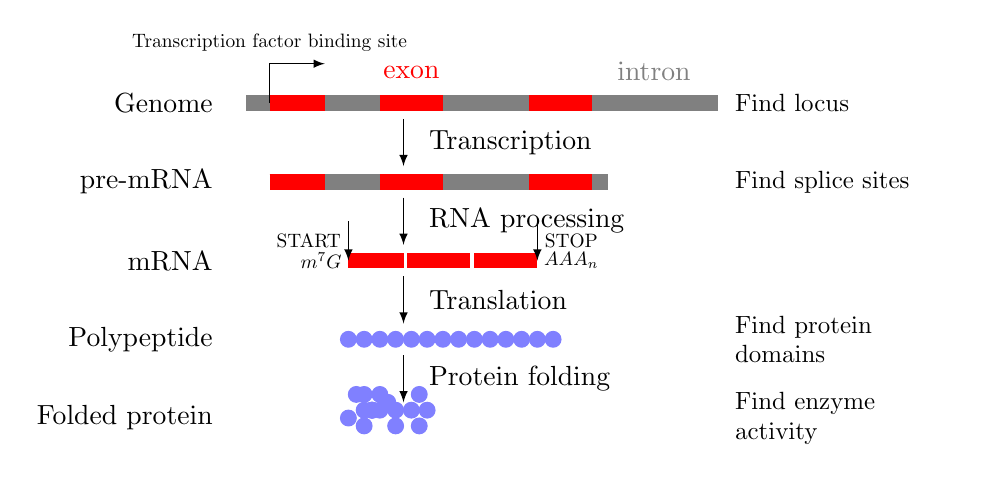
\begin{tikzpicture}
\node [color=black,anchor=east] at (-0.3cm,0cm) {Genome};
\draw [line width=0.2cm, anchor=west,color=gray]  (0cm,0cm) -- (6cm,0cm);
\draw [line width=0.2cm, anchor=west,color=red]  (0.3cm,0cm) --  (1cm,0cm);
\draw [line width=0.2cm, anchor=west,color=red]  (1.7cm,0cm) --node [color=red,above=0.1cm] {exon} (2.5cm,0cm);
\draw [line width=0.2cm, anchor=west,color=red]  (3.6cm,0cm) -- node [color=gray,above=0.4cm,right=0.5cm] {intron} (4.4cm,0cm);
\draw [-latex] (0.3cm,0cm) -- (0.3cm,0.5cm) node [scale=0.7,above=0.1cm] {Transcription factor binding site} -- (1cm,0.5cm);

\draw [-latex,] (2cm, -0.2cm) -- node [right=0.2cm] {Transcription} (2cm,-0.8cm);
\node [color=black,anchor=west,text width=3cm,scale=0.9] at (6.1cm,0cm) {Find locus};

\begin{scope}[yshift=-1cm]
\node [color=black,anchor=east] at (-0.3cm,0cm) {pre-mRNA};
\draw [line width=0.2cm, anchor=west,color=gray] (0.3cm,0cm) -- (4.6cm,0cm);
\draw [line width=0.2cm, anchor=west,color=red]  (0.3cm,0cm) -- (1cm,0cm);
\draw [line width=0.2cm, anchor=west,color=red]  (1.7cm,0cm) -- (2.5cm,0cm);
\draw [line width=0.2cm, anchor=west,color=red]  (3.6cm,0cm) -- (4.4cm,0cm);
\draw [-latex,] (2cm, -0.2cm) -- node [right=0.2cm] {RNA processing} (2cm,-0.8cm);
\node [color=black,anchor=west,text width=3cm,scale=0.9] at (6.1cm,0cm) {Find splice sites};
\end{scope}

\begin{scope}[yshift=-2cm]
\node [color=black,anchor=east] at (-0.3cm,0cm) {mRNA};
\node [color=black,anchor=east,scale=0.7] at (1.3cm,0cm) {$m^{7}G$};
\draw [line width=0.2cm, anchor=west,color=red]  (1.3cm,0cm) -- (2cm,0cm);
\draw [line width=0.2cm, anchor=west,color=red]  (2.05cm,0cm) -- (2.85cm,0cm);
\draw [line width=0.2cm, anchor=west,color=red]  (2.9cm,0cm) -- (3.7cm,0cm);
\node [color=black,anchor=west,scale=0.7] at (3.7cm,0cm) {$AAA_{n}$};
\draw [latex-,color=black] (1.3cm,0cm) --  node [scale=0.7,left=0.01cm] {START} (1.3cm,0.5cm);
\draw [latex-,color=black] (3.7cm,0cm) -- node [scale=0.7,right=0.01cm] {STOP} (3.7cm,0.5cm) ;
\draw [-latex,] (2cm, -0.2cm) -- node [right=0.2cm] {Translation} (2cm,-0.8cm);
\end{scope}

\begin{scope}[yshift=-3cm]
\node [anchor=east] at (-0.3cm,0cm) {Polypeptide};
\draw [fill=blue!50!white, color=blue!50!white] (1.3cm,0cm) circle (0.1cm);
\draw [fill=blue!50!white, color=blue!50!white] (1.5cm,0cm) circle (0.1cm);
\draw [fill=blue!50!white, color=blue!50!white] (1.7cm,0cm) circle (0.1cm);
\draw [fill=blue!50!white, color=blue!50!white] (1.9cm,0cm) circle (0.1cm);
\draw [fill=blue!50!white, color=blue!50!white] (2.1cm,0cm) circle (0.1cm);
\draw [fill=blue!50!white, color=blue!50!white] (2.3cm,0cm) circle (0.1cm);
\draw [fill=blue!50!white, color=blue!50!white] (2.5cm,0cm) circle (0.1cm);
\draw [fill=blue!50!white, color=blue!50!white] (2.7cm,0cm) circle (0.1cm);
\draw [fill=blue!50!white, color=blue!50!white] (2.9cm,0cm) circle (0.1cm);
\draw [fill=blue!50!white, color=blue!50!white] (3.1cm,0cm) circle (0.1cm);
\draw [fill=blue!50!white, color=blue!50!white] (3.3cm,0cm) circle (0.1cm);
\draw [fill=blue!50!white, color=blue!50!white] (3.5cm,0cm) circle (0.1cm);
\draw [fill=blue!50!white, color=blue!50!white] (3.7cm,0cm) circle (0.1cm);
\draw [fill=blue!50!white, color=blue!50!white] (3.9cm,0cm) circle (0.1cm);
\draw [-latex,] (2cm, -0.2cm) -- node [right=0.2cm] {Protein folding} (2cm,-0.8cm);
\node [color=black,anchor=west,text width=3cm,scale=0.9] at (6.1cm,0cm) {Find protein\\ domains};
\end{scope}

\begin{scope}[yshift=-4cm]
\node [anchor=east] at (-0.3cm,0cm) {Folded protein};
\draw [fill=blue!50!white, color=blue!50!white] (1.3cm,0cm) circle (0.1cm);
\draw [fill=blue!50!white, color=blue!50!white] (1.5cm,0.1cm) circle (0.1cm);
\draw [fill=blue!50!white, color=blue!50!white] (1.7cm,0.3cm) circle (0.1cm);
\draw [fill=blue!50!white, color=blue!50!white] (1.5cm,0.3cm) circle (0.1cm);
\draw [fill=blue!50!white, color=blue!50!white] (1.6cm,0.1cm) circle (0.1cm);
\draw [fill=blue!50!white, color=blue!50!white] (1.5cm,-0.1cm) circle (0.1cm);
\draw [fill=blue!50!white, color=blue!50!white] (1.6cm,0.1cm) circle (0.1cm);
\draw [fill=blue!50!white, color=blue!50!white] (1.4cm,0.3cm) circle (0.1cm);
\draw [fill=blue!50!white, color=blue!50!white] (1.6cm,0.1cm) circle (0.1cm);
\draw [fill=blue!50!white, color=blue!50!white] (1.7cm,0.1cm) circle (0.1cm);
\draw [fill=blue!50!white, color=blue!50!white] (1.8cm,0.2cm) circle (0.1cm);
\draw [fill=blue!50!white, color=blue!50!white] (1.9cm,0.1cm) circle (0.1cm);
\draw [fill=blue!50!white, color=blue!50!white] (1.9cm,-0.1cm) circle (0.1cm);
\draw [fill=blue!50!white, color=blue!50!white] (2.1cm,0.1cm) circle (0.1cm);
\draw [fill=blue!50!white, color=blue!50!white] (2.2cm,0.3cm) circle (0.1cm);
\draw [fill=blue!50!white, color=blue!50!white] (2.3cm,0.1cm) circle (0.1cm);
\draw [fill=blue!50!white, color=blue!50!white] (2.2cm,-0.1cm) circle (0.1cm);
\node [color=black,anchor=west,text width=3cm,scale=0.9] at (6.1cm,0cm) {Find enzyme\\ activity};
\end{scope}


\end{tikzpicture}
\end{figure}
\end{center}
\end{frame}
\begin{frame}[label=sec-4-1-7]{Gene ontologies}
\begin{center}

\begin{figure}[htb]
\centering
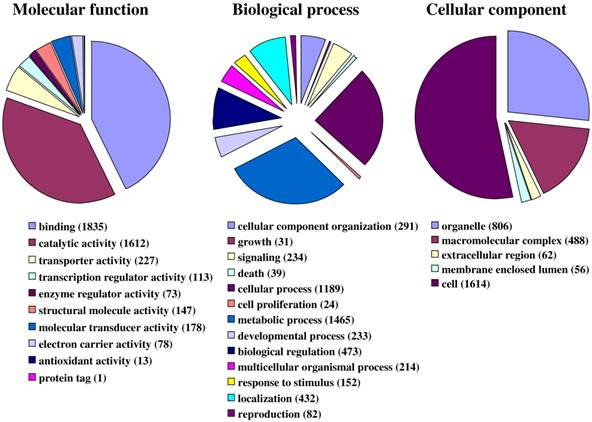
\includegraphics[width=8cm]{Jacquin-Joly-Fig1.jpg}
\caption{GO terms of unigenes in a moth genome}
\end{figure}

\tiny{\citep{Jacquin2012}}
\end{center}
\end{frame}



\begin{frame}[label=sec-4-1-8]{Cloud of GO term enrichments}
\begin{figure}[htb]
\centering
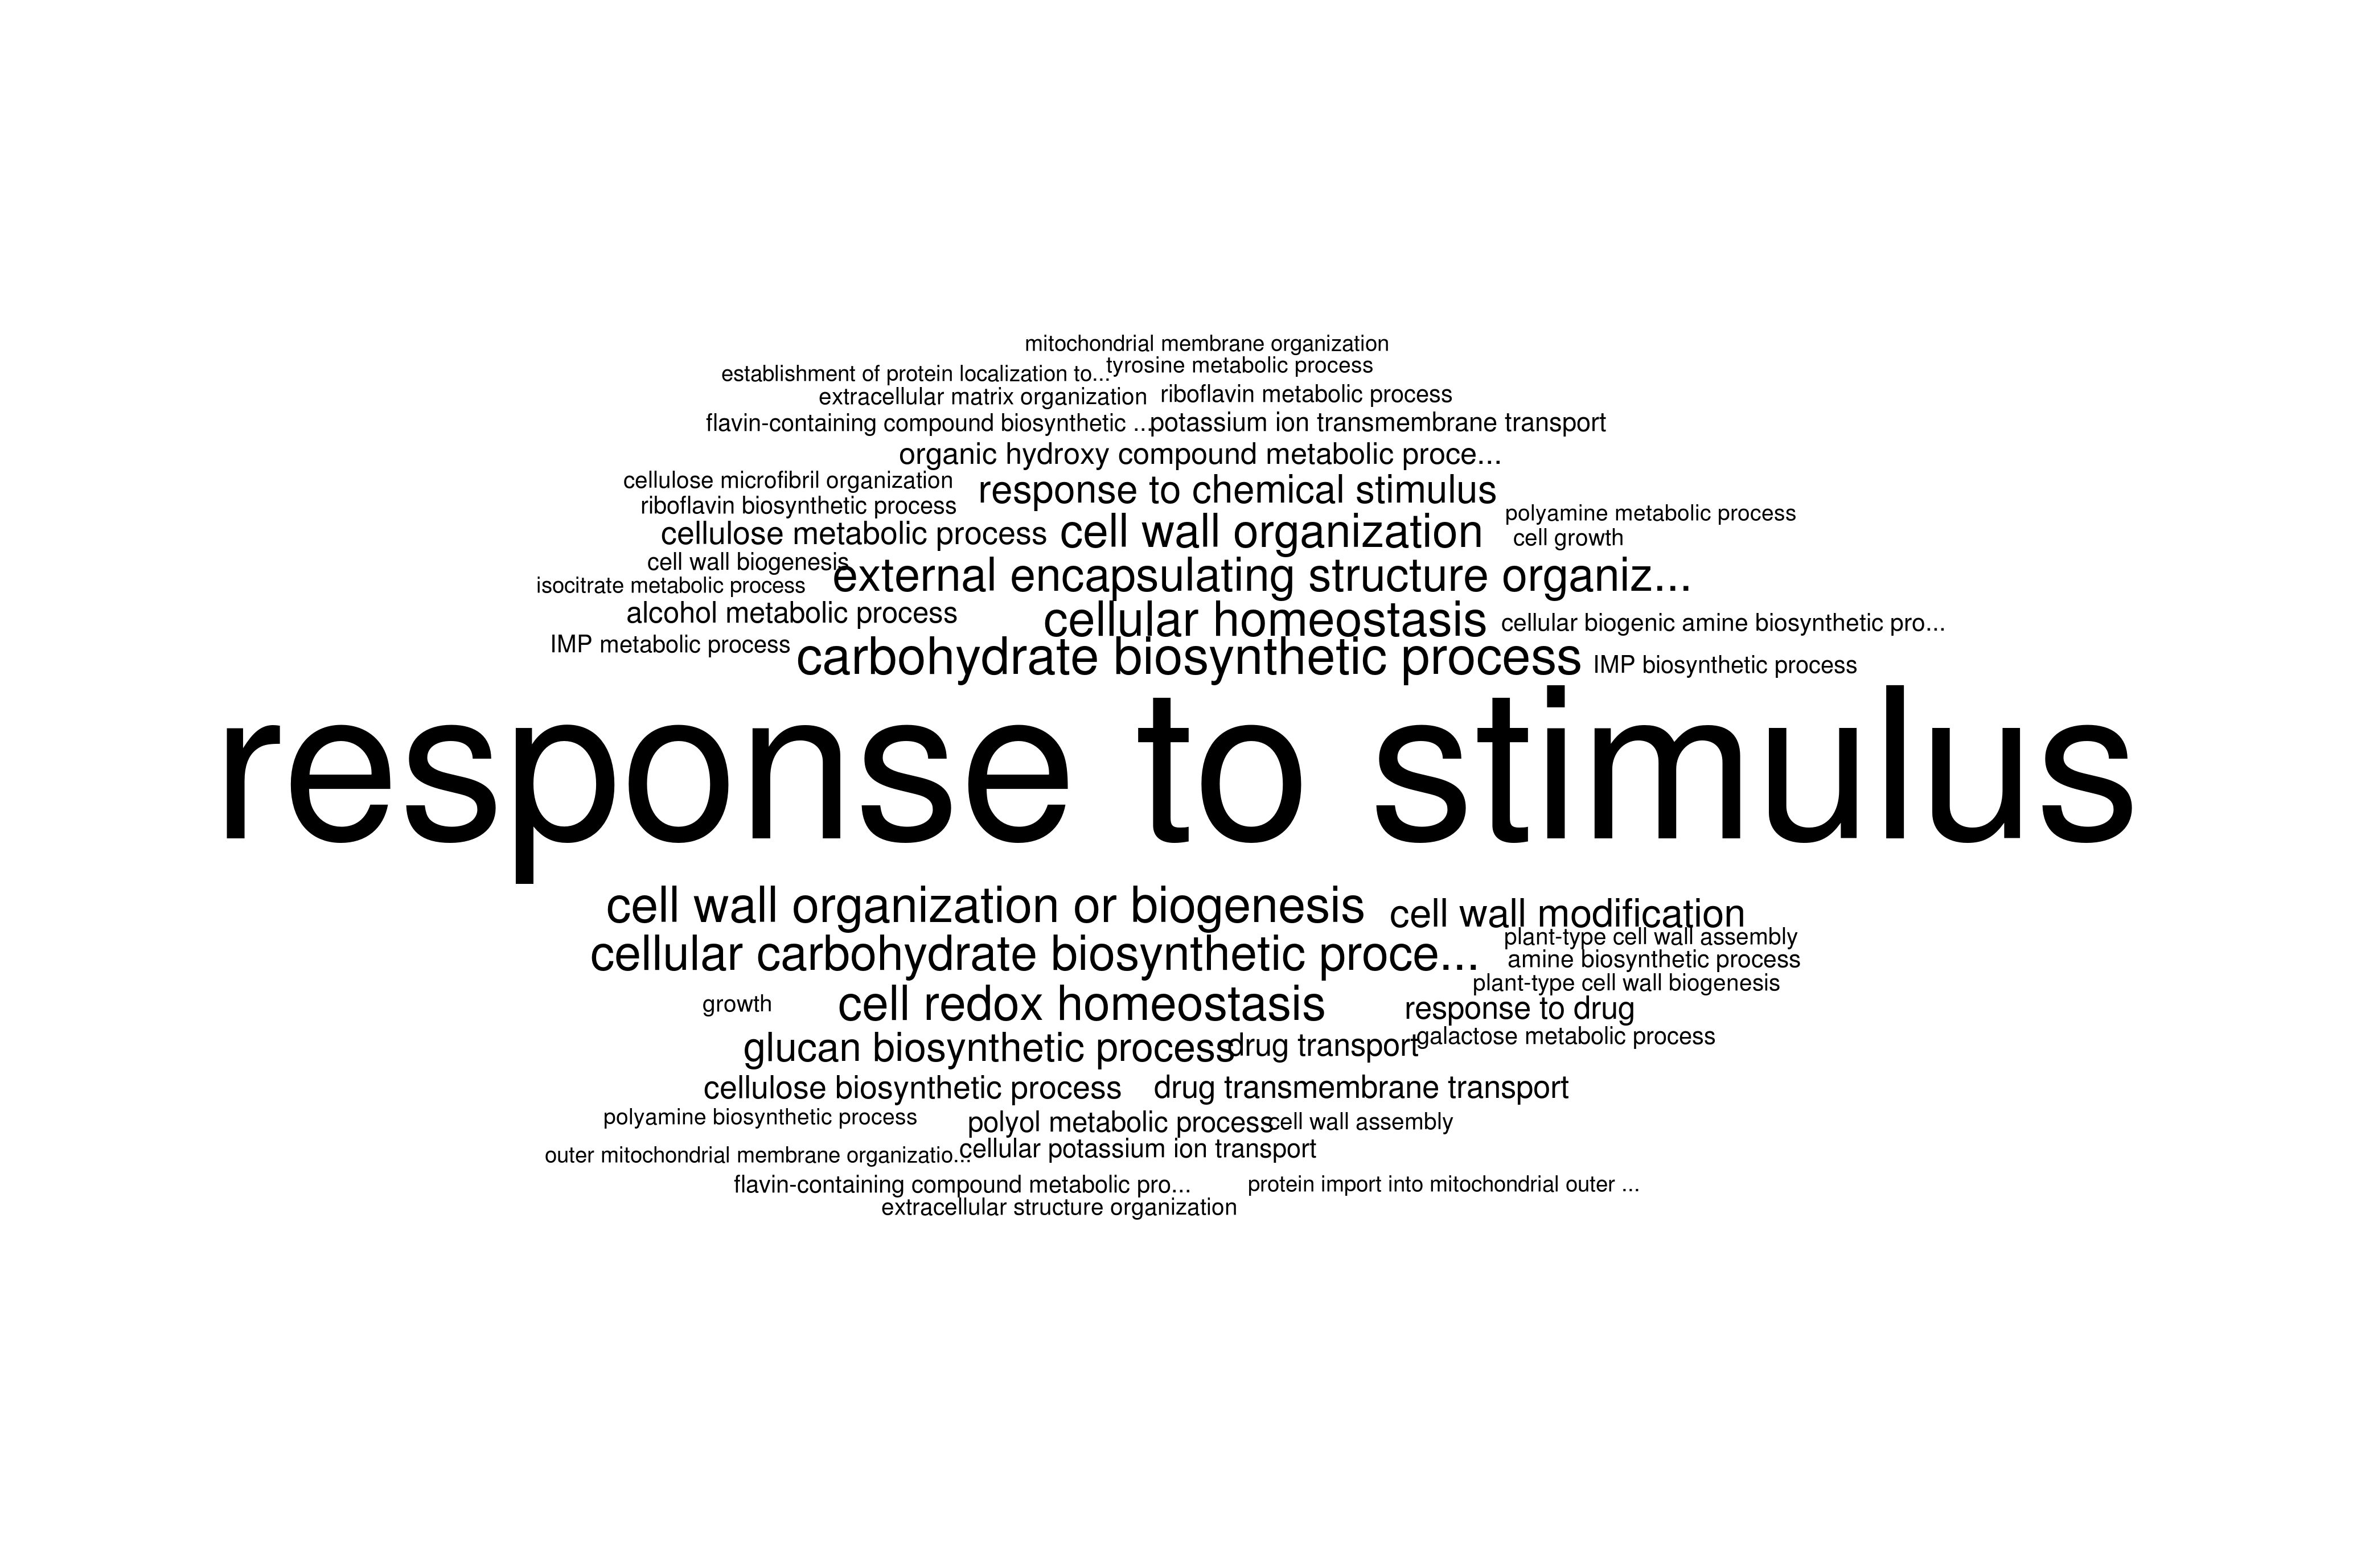
\includegraphics[width=9cm]{t3c1BPincreased.png}
\caption{Term cloud of heat-responsive functions in seagrass}
\end{figure}
\end{frame}

\section{Plan}
\label{sec-5}
\subsection{Bioinformatics-Practical}
\label{sec-5-1}
\begin{frame}[label=sec-5-1-1]{Bioinformatics-Practical}
\begin{itemize}
\item Unix Tools (Martin)
\item Trimming and Quality Control (Martin)
\item Genome Assembly (Alexander)
\item Mapping and Variant Calling (Martin)
\end{itemize}
\end{frame}
\begin{frame}[allowframebreaks]{References}
\raggedright
\printbibliography[sorting=nty,heading=bibnumbered]
\end{frame}
% Emacs 24.5.1 (Org mode 8.3beta)
\end{document}